\begin{anexosenv}

\partanexos

\chapter{Códigos do MATLAB}
    \begin{lstlisting}
            
        %%
% Feito por: Fernanda Muro e Daniela Dias
% Projeto integrador 2


clc;
clear all
close all
% CALCULO ESTRUTURAL DO RADAR DE PREVENÇÃO DE ACIDENTES RaDOP

%As análises foram feitas vendo o projeto na vista lateral, considerando:
%parte da frente o projeto (bateria, caixa e camera) à esquerda e a parte 
%traseira do projeto (painel solar) à direita. A antena ficou neutra em
%relação à sua posição ao eixo de simetria.

%No caso:
%{
%Projeto visto de frente

            A (ntena)           
            |    (Atras tem o paines solar que não deu pra desenhar)
           ----    
          |    |-* Caixa vista de frente dando suporta a camera
          |____|
           |  | Eixos
           |  |
           ____
          |____| bateria


Projeto vista lateral (considerada para essa rotina)

              A (ntena)
              |
             ___    
      caixa |  *| __
            |___|/_/ Painel Solar
                |
                | eixos de sustentação
              __|
             |__| Bateria

%%%% As distancias usadas para calcular os momentos que cada componente gera
foram usadas a partir dessa referencia ultilizando os centroides de cada
componente individualmente e as distancias que esse centroide poderia estar
da estrutura.
%%%% Podemos ver que o painel solar está no lugar oposto à caixa e a
bateria, por isso, ao colocar a sua largura la em baixo, colocar com o
sinal negativo pra ele poder calcular os momentos certos. As equações foram
adaptadas para esse cenário.
%}
%%%%%%%%%%%%%%%%%%%%%%%%%%%%%%%%

%% Condições climáticas

vent_med = input('Velocidade media do vento na regiao: '); %m/s
ca = 1.2; %Coeficiente de arrasto com valor em tabela, por isso é fixo.
S1 = 1; S2 = 0.9; S3 = 1; %Critérios que contabilizam na velocidade do vento de projeto
vk = 2*(vent_med*S1*S2*S3); %Vento de projeto; fator 2 adicionado à 
%torção causada pelo vento %fator de segurança de torção
q = (vk^2)*0.613; %Pressão dinamica

%%

%Adiquirindo os dados geométricos e calculando o centroide dos componentes

Z = 'Quantos componentes vão alocados na estrutura?';
disp(Z)

num_comp = input(' ');

%{
nome_comp = [];
peso_comp = [];
dist_vert = [];
dist_hori = [];
posX_comp = [];
posY_comp = [];
posZ_comp = [];
%}

%Armazeando os nomes, o peso e a distancia que os componentes 
%estarão da haste
for i=1:num_comp
    nome_comp{i} = input('Digite o nome do componente: ','s');
    peso_comp{i} = input('Digite o peso do componente (kg): ');
    comp_comp{i} = input('Digite o comprimento do componente (mm): '); %X
    altu_comp{i} = input('Digite a altura do componente (mm): '); %Y
    larg_comp{i} = input('Digite a largura do componente (mm): '); %Z
%     altu_psin_comp{i} = input('Digite a altura do painel solar inclinado (mm): '); 
%     larg_psin_comp{i} = input('Digite a largura do painel solar inclinado (mm): '); %Z
    %Distancia dos componentes ao eixo de simetria da estrutura no geral
    dist_hori{i} = input('Digite a distancia horizontal do componente aos eixos estruturais (mm): ');
    dist_vert{i} = input('Digite a distancia vertical do componente ao chao (mm): '); 
end


%{
%Painel solar
disp('Insira as propriedades do painel solar')
nome_painel = input('Digite o nome do componente: ');
peso_painel = input('Digite o peso do componente (kg): ');
comp_painel = input('Digite o comprimento do componente (mm): ');
altu_painel = input('Digite a altura do componente (mm): ');
larg_painel = input('Digite a largura do componente (mm): ');
dhori_painel = input('Digite a distancia horizontal do componente aos eixos estruturais (mm): ');
dvert_painel = input('Digite a distancia vertical do componente ao chao (mm): ');
%}

%Convertendo as distancias para metro
for i=1:num_comp
   comp_comp{i} = comp_comp{i}*10^-3;
   altu_comp{i} = altu_comp{i}*10^-3;
   larg_comp{i} = larg_comp{i}*10^-3;
   dist_hori{i} = dist_hori{i}*10^-3;
   dist_vert{i} = dist_vert{i}*10^-3;
   %Painel solar
%    altu_psin_comp{i} = altu_psin_comp{i}*10^-3; 
%    larg_psin_comp{i} = larg_psin_comp{i}*10^-3;
end

%Calculando o centroide dos componentes
%Partindo que todos os componentes tem seção transversal retangular

%Calculo do centroide (m)
for i=1:num_comp
    %Calculo do centroide em relação à Y (altura)
    centroideY{i} = altu_comp{i}/2;
    %Calculo do centroide em relação à X (comprimento)
    centroideX{i} = larg_comp{i}/2;
    %Calculo do centroide em relação à Z (largura)
    centroideZ{i} = comp_comp{i}/2;
    %Calculo do centroide do painel inclinado
%     centroide_ps_Y{i} = altu_psin_comp{i}/2
%     centroide_ps_X{i} = larg_psin_comp{i}/2;
%     
end

%Mostrando as informações
for i=1:num_comp
    disp(nome_comp(i));    
    disp(peso_comp(i));
    disp(centroideY(i));
    disp(centroideX(i));
    disp(centroideZ(i));
    %disp(centroide_ps_X(i));
    %disp(centroide_ps_y(i));
end

%{
%Convertendo as distancias para metro - painel solar
   comp_painel = comp_painel*10^-3;
   altu_painel = altu_painel*10^-3;
   larg_painel = larg_painel*10^-3;
   dhori_painel = dhori_painel*10^-3;
   dvert_painel = dvert_painel*10^-3;
%Area do painel que a força do vento 
area_painel = comp*painel*altu_painel; 
%}
%% Calculando as forças atuantes na estrutura;

%Calculando a força peso dos componentes
g = 9.81;
for i=1:num_comp
    fpes_comp{i} = peso_comp{i}*g;
end

%Calculando a força do vento nos componentes
for i=1:num_comp
    fven_comp{i} = q*ca*comp_comp{i}*altu_comp{i};
end
    
%{
for i=1:num_comp
    fven_comp{i} = -(q*ca*comp_comp{i}*altu_comp{i});
end
%}
%comp_comp{i}*altu_comp{i} é a área onde o vento bate a 90º 

%{
A força do vento é calculada segundo as normas ABNT 6123 e 14228
Segundo a norma 6123 o valor da velocidade do vento a ser considerado é Vo
= 35m/s
Vk = VoxS1xS2xS3
Si, s2 e s3 são valores geográficos fixos de acordo com a norma
eles são: S1 = 1
s2 = 0.9
s3 = 1
%}


%% Calculando as reações de esforços externo

%Esforços externos 
%Para um portico vertical: 
t_nor = 0; %va = esforço normal
t_cor = 0; %ha = esforço cortante
map = 0; %map = momento causado pela força peso
mav = 0; %mav = momento causado pela força do vento nas componentes;
mt = 0; %mt = mav + map


%Calculo t_nor
for i=1:length(fpes_comp)
    t_nor = t_nor + fpes_comp{i}; %todas mesmo sentido
end
t_nor


%Calculando Ha - tensão de cisalhamento
t_cor = 0;
for i=1:length(fven_comp)
    t_cor = t_cor + fven_comp{i}; %todas mesmo sentido
end


%O calculo do momento vai levar em cosideração duas forças: a força peso
%dos componentes e a força do que o vento exerce neles. A FORÇA DO VENTO
%NÃO ESTÁ SENDO CONSIDERADA NOS PILARES ESTRUTURAIS.

%calculando Ma(N*m)

%Calculando as distancias entre o centroide dos componentes e 
%a estrutura; posição estrutura = 0;

%Calculo das distancias dos componentes em relação à estrutura e ao seu
%centroide. 

for i=1:num_comp
       %{
    %Distancia total do centroide do componente à estrutura levando 
    em conta se ele está longe com apoio.
    %}
    dt_hori{i} = dist_hori{i} + centroideX{i}; 
    dt_vert{i} = dist_vert{i} + centroideY{i};
    
end
   
 %calculando o momento parcial gerado pela força peso
    for i=1:length(fpes_comp)
        map = map + fpes_comp{i}*dt_hori{i};
    end
 
 %Calculando o momento parcial gerado pela força do vento
    for i=1:length(fven_comp)
       mav = mav + fven_comp{i}*dt_vert{i};
    end

%Calculando o momento parcial no sentido do momento do pesos

%Reação do momento Ma
mt = map + mav

%% MECSOL 2 E PROJETO ESTRUTURAL

%Declaração das variáveis utilizadas no projeto


%Material
nome = input('Digite o material escolhido: ', 's');
%disp(nome);
X = 'Colocar as propriedades mecanicas do material escolhido com as unidades de acordo com as tabelas postadas no drive';
disp(X)
%}

%Adquirindo os valores das propriedades do material


%Peso especifico do material (g/cc)
peso_esp = input('Peso especifico do material: ');
%Conversão de unidades 
peso_esp = peso_esp*1000; %kg/m^3
%Valor da tensão ultima em MPa; Utilizada no calculo das tensões normais
%Valor da tensao de escoamento em MPa
ten_esc = input('Valor da tensao de escoamento (MPa): ');
% %Valor da tensão da tensão ultima
% ten_ult = input('Valor da tensao ultima (MPa): ');
% %Valor do módulo de elasticidade MPa
mod_elas = input('Valor do modulo de elasticidade (MPa): ');
%fator de segurança
CS = input('Valor do coeficiente de seguranca do projeto: '); 

%Calculo da força peso da haste
fph = peso_esp*g;

%{
As tensões utilizadas para análise e projeto da estrutura são:
a) Tensões normais causadas por: carregamentos axiais e momentos;
b) Tensões de cisalhamento causadas por: momento de torção e carregamentos
transversais. 

tnor = (P/A) + (Mmax*y)/I; e 
tcis = (T*ro)/J + VmaxQ/It

Sabendo onde elas são máximas (no engaste), é possível calcular uma
estrutura segura para os esforços atuantes.

O momento máximo da estrutura no trecho (0<=x,=centroide(bateria))
Mmax(x) = ha(x) + mt;
O esforço cortante máximo na estrutura, no mesmo trecho, é:
Vmax(x) = ha;

Calcular os esforços combinados e analisar qual material será o mais
adequado
%}

%Calculo das tensões
%Tensões estruturais
%{
Mz = mt; O momento em Z é o momento interno reagente ao momento externo;
Ha = v; Tensão de cisalhamento é o esforço cortante reagente ao enforço
cortante externo;
%}

%Declaração das tensões estruturais
mz = mt;
t_nor;
t_cor;
%Declaração das propriedades da geometria

%Axiais 
%{
ten_nor = ((mz*dr)/I)- P/A; %Momento tracionando e força normal comprimindo;
ten_cis = (ha*q)/(I*r); %NÃO HÁ MOMENTO TORSOR POIS NÃO HÁ TORSÃO
v = força cortante na sessão transversal;
q = momento estatico; I = momento de inércia; t = espessura da geometria

ten_nor_Mz = (4*mz*r)/(pi*R^4) - pa/(pi*r^2)

ten_cis_va = (2*va)/(3*(r^3)*pi)
%} 

re= 0.005:0.001:0.5; %raio externo em m;
ri= 0.0025; %raio interno em m;
r=re-ri;
t_normal = (4*mz)./(pi*r.^4) - (t_nor+fph)./(pi*r.^2);
%((2*Mz*b)./pi*(r).^4) +((2*Mx*b)./pi*(r).^4) - g*(p1+p2+p3+p4+ph)./(pi*r.^2);
t_cis = (2*t_cor)./(3*(pi*r.^3));

tnor_adm=ten_esc/CS; %tensão de flexão máxima admissível
tcis_adm=ten_esc/(2*CS); %tensão de cisalhamento máxima admissível

%{
%re e ri = raios externos e internos, respectivamente.
%Calculo das tensões
    re= 0.005:0.001:0.5; %raio externo em m;
    ri= 0.0025; %raio interno em m;
    r = re-ri;

tnormal_adm = ten_esc/CS; %tensão de flexão máxima admissível
tcisa_adm = ten_esc/2*CS; %tensão de cisalhamento máxima admissível
%}


plot(2*re,t_normal/10^6);
title('relação de diâmetro externo com a tensão de flexão')
xlabel('Diâmetro (m)')
ylabel('Tensão (MPa)')
hold on
plot(2*re,tnor_adm*ones(size(re)),'--')


figure(2)
plot(2*re,t_cor);
title('relação de diâmetro externo com a tensão de cisalhamento')
xlabel('Diâmetro (m)')
ylabel('Tensão (MPa)')
hold on
plot(2*re,tcis_adm*ones(size(re)),'--')

            
    \end{lstlisting}
    
\chapter{Plantas dos Componentes}

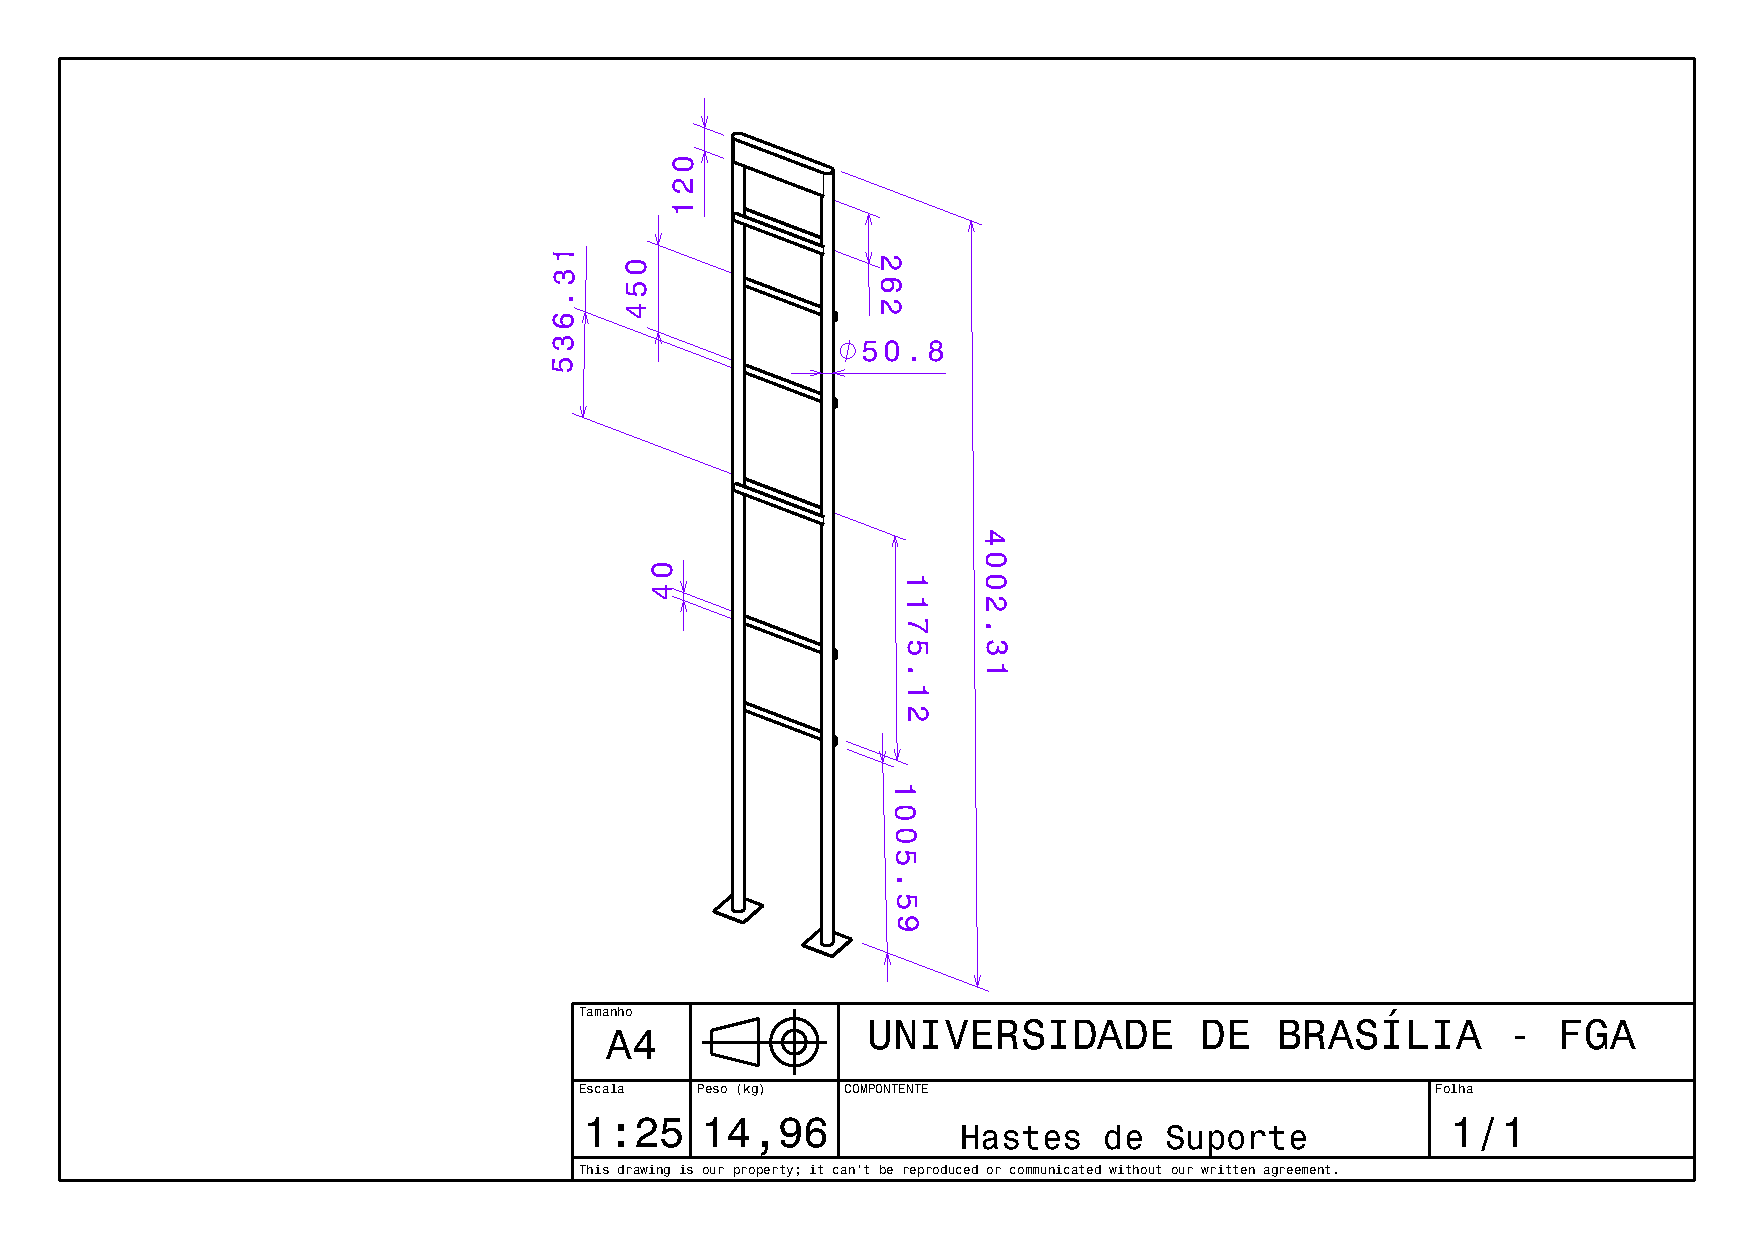
\includepdf[angle=90]{Haste.pdf}
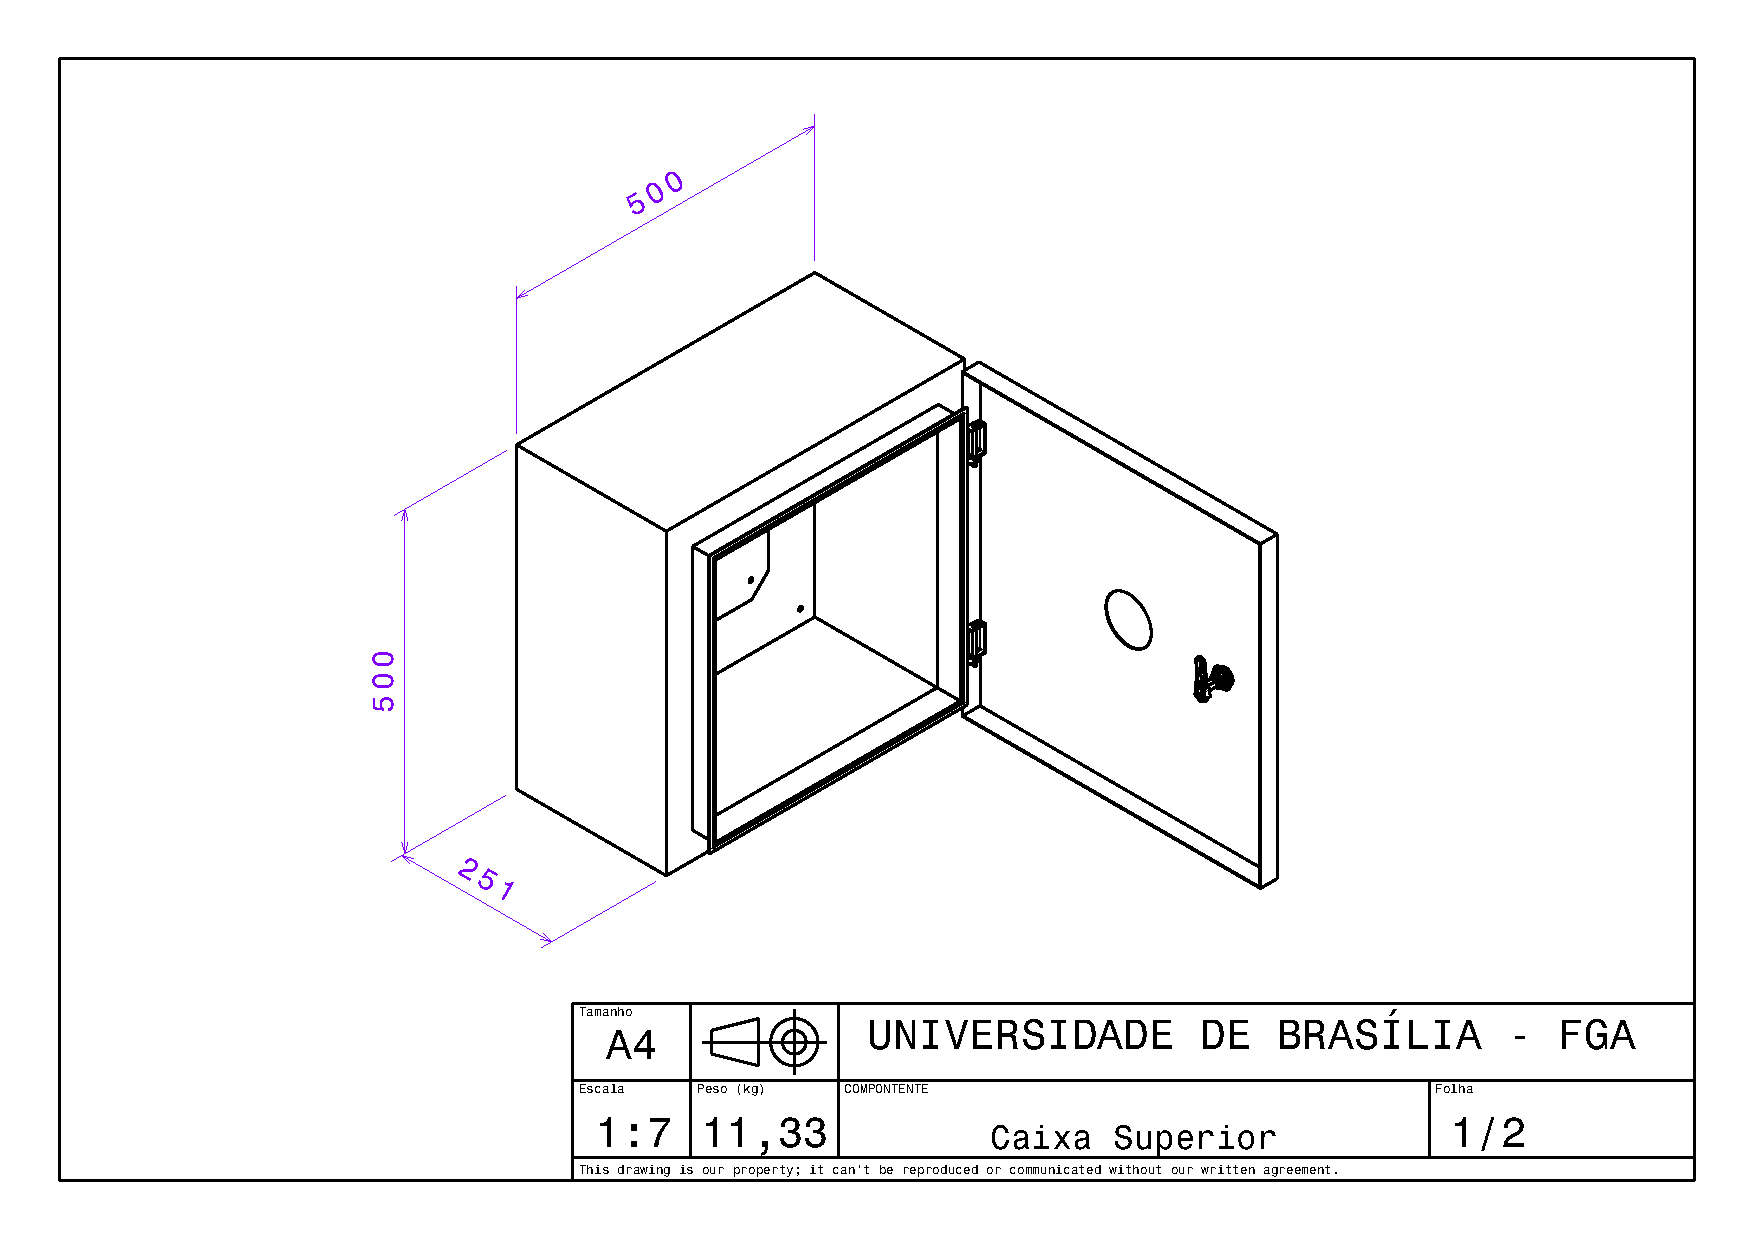
\includepdf[angle=90]{CaixaSup1.pdf}
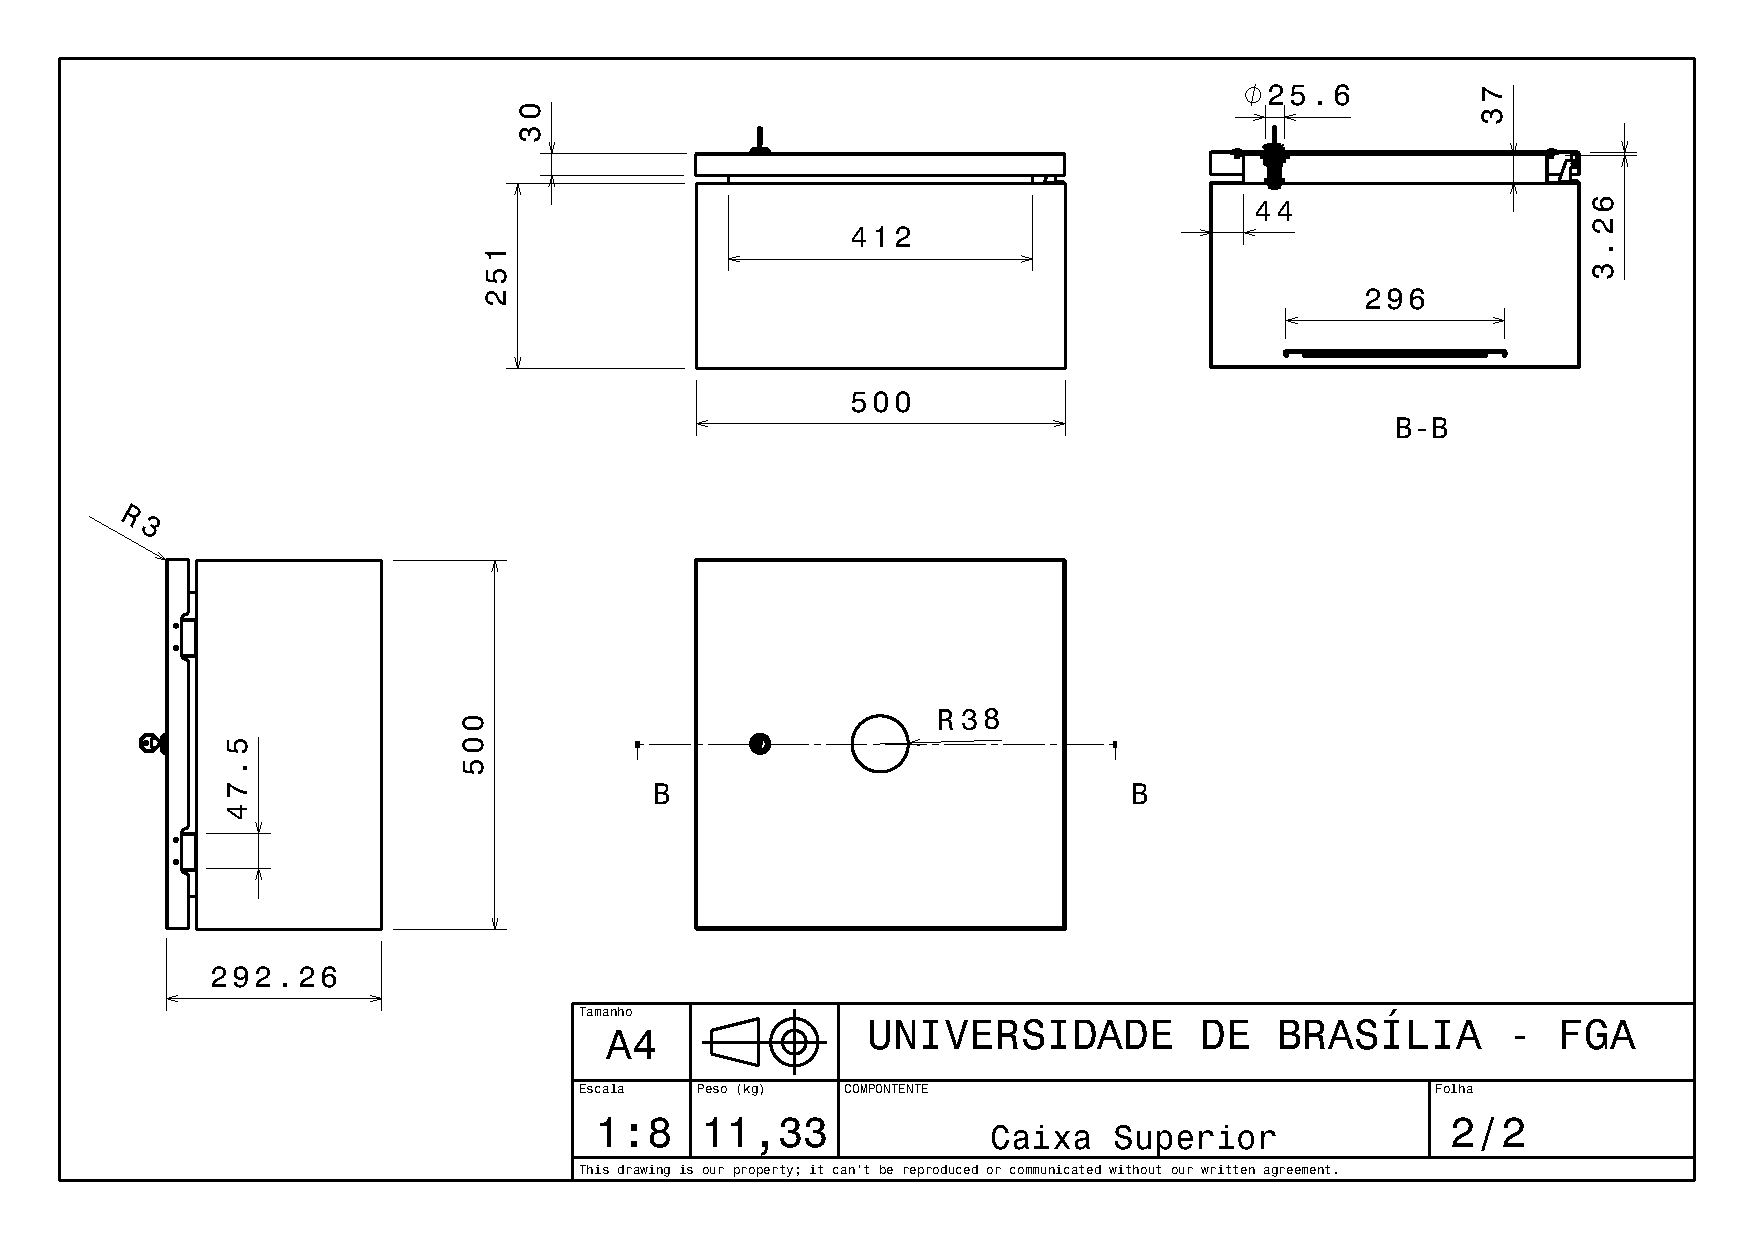
\includepdf[angle=90]{CaixaSup2.pdf}
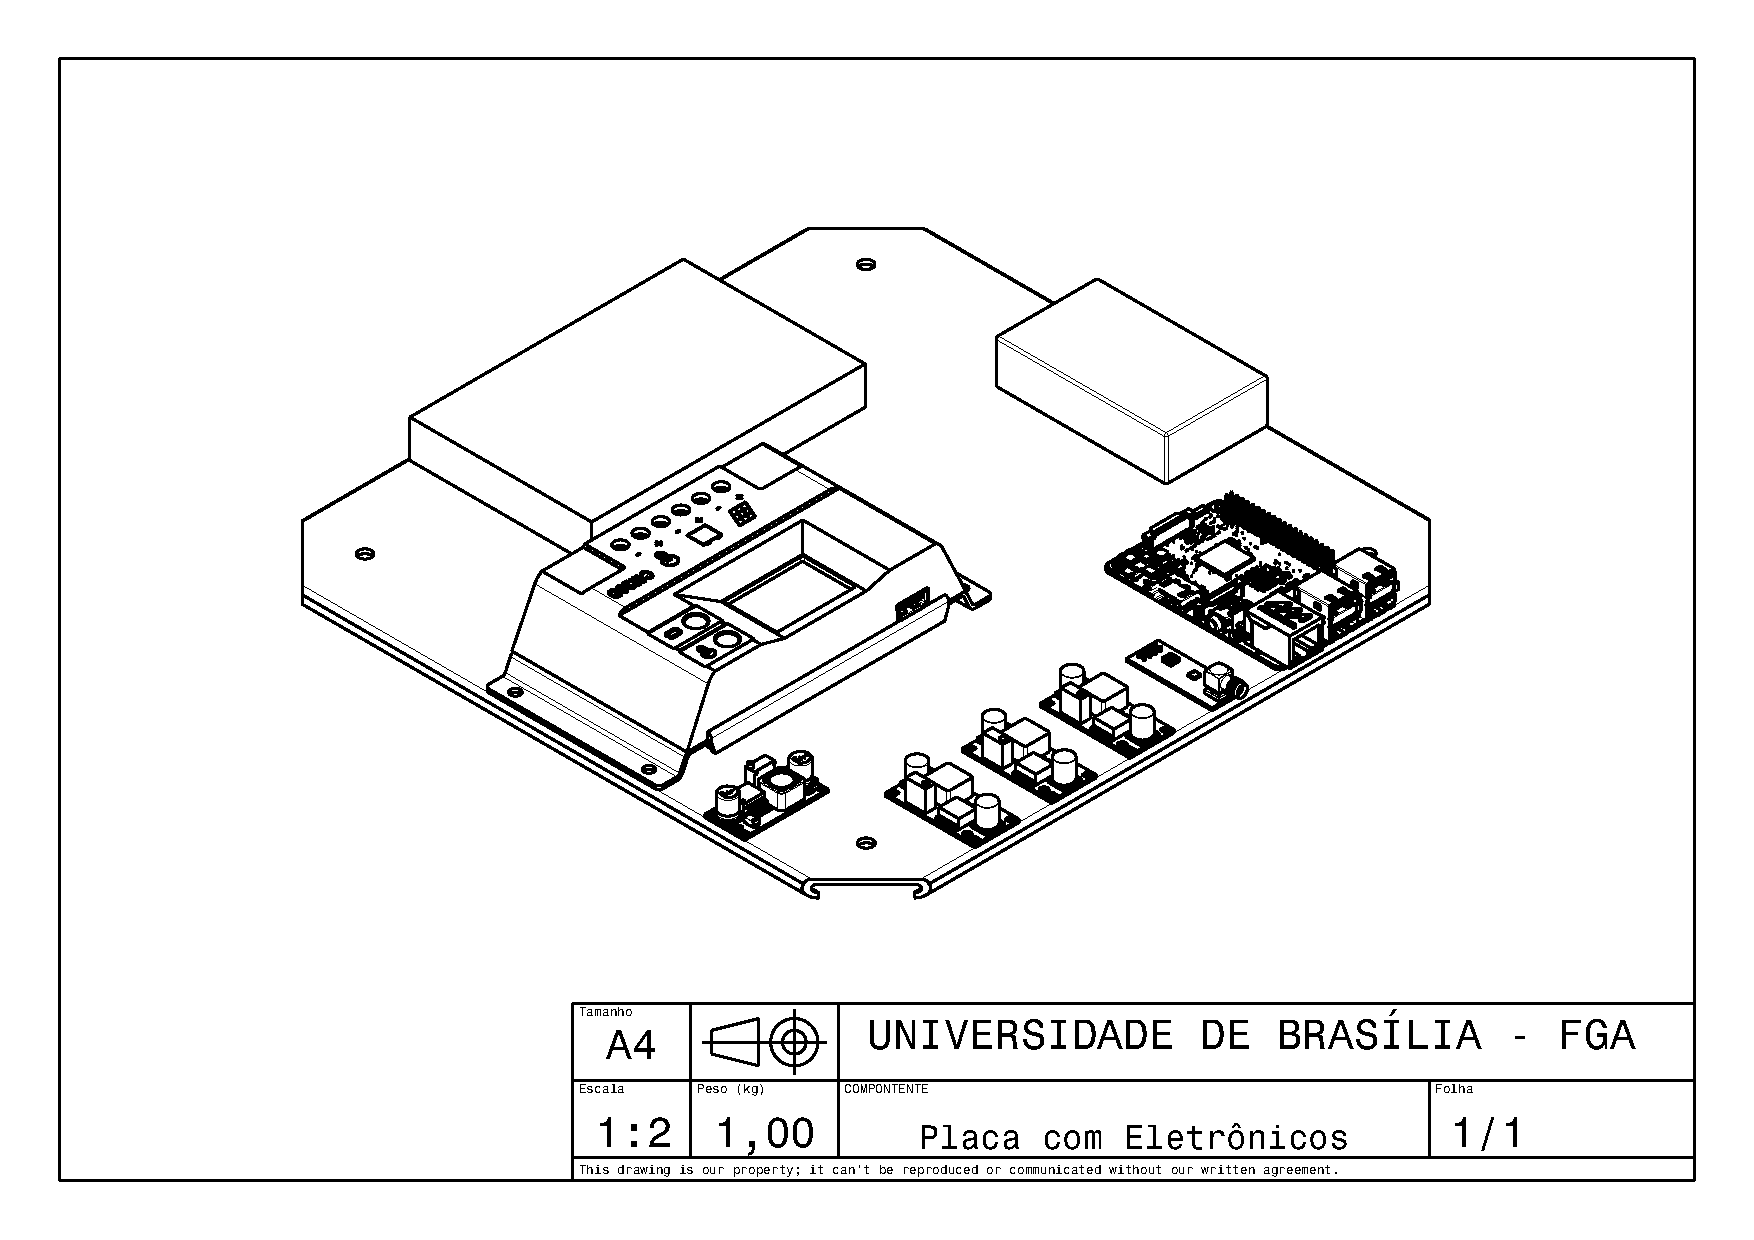
\includepdf[angle=90]{Eletronicos.pdf}
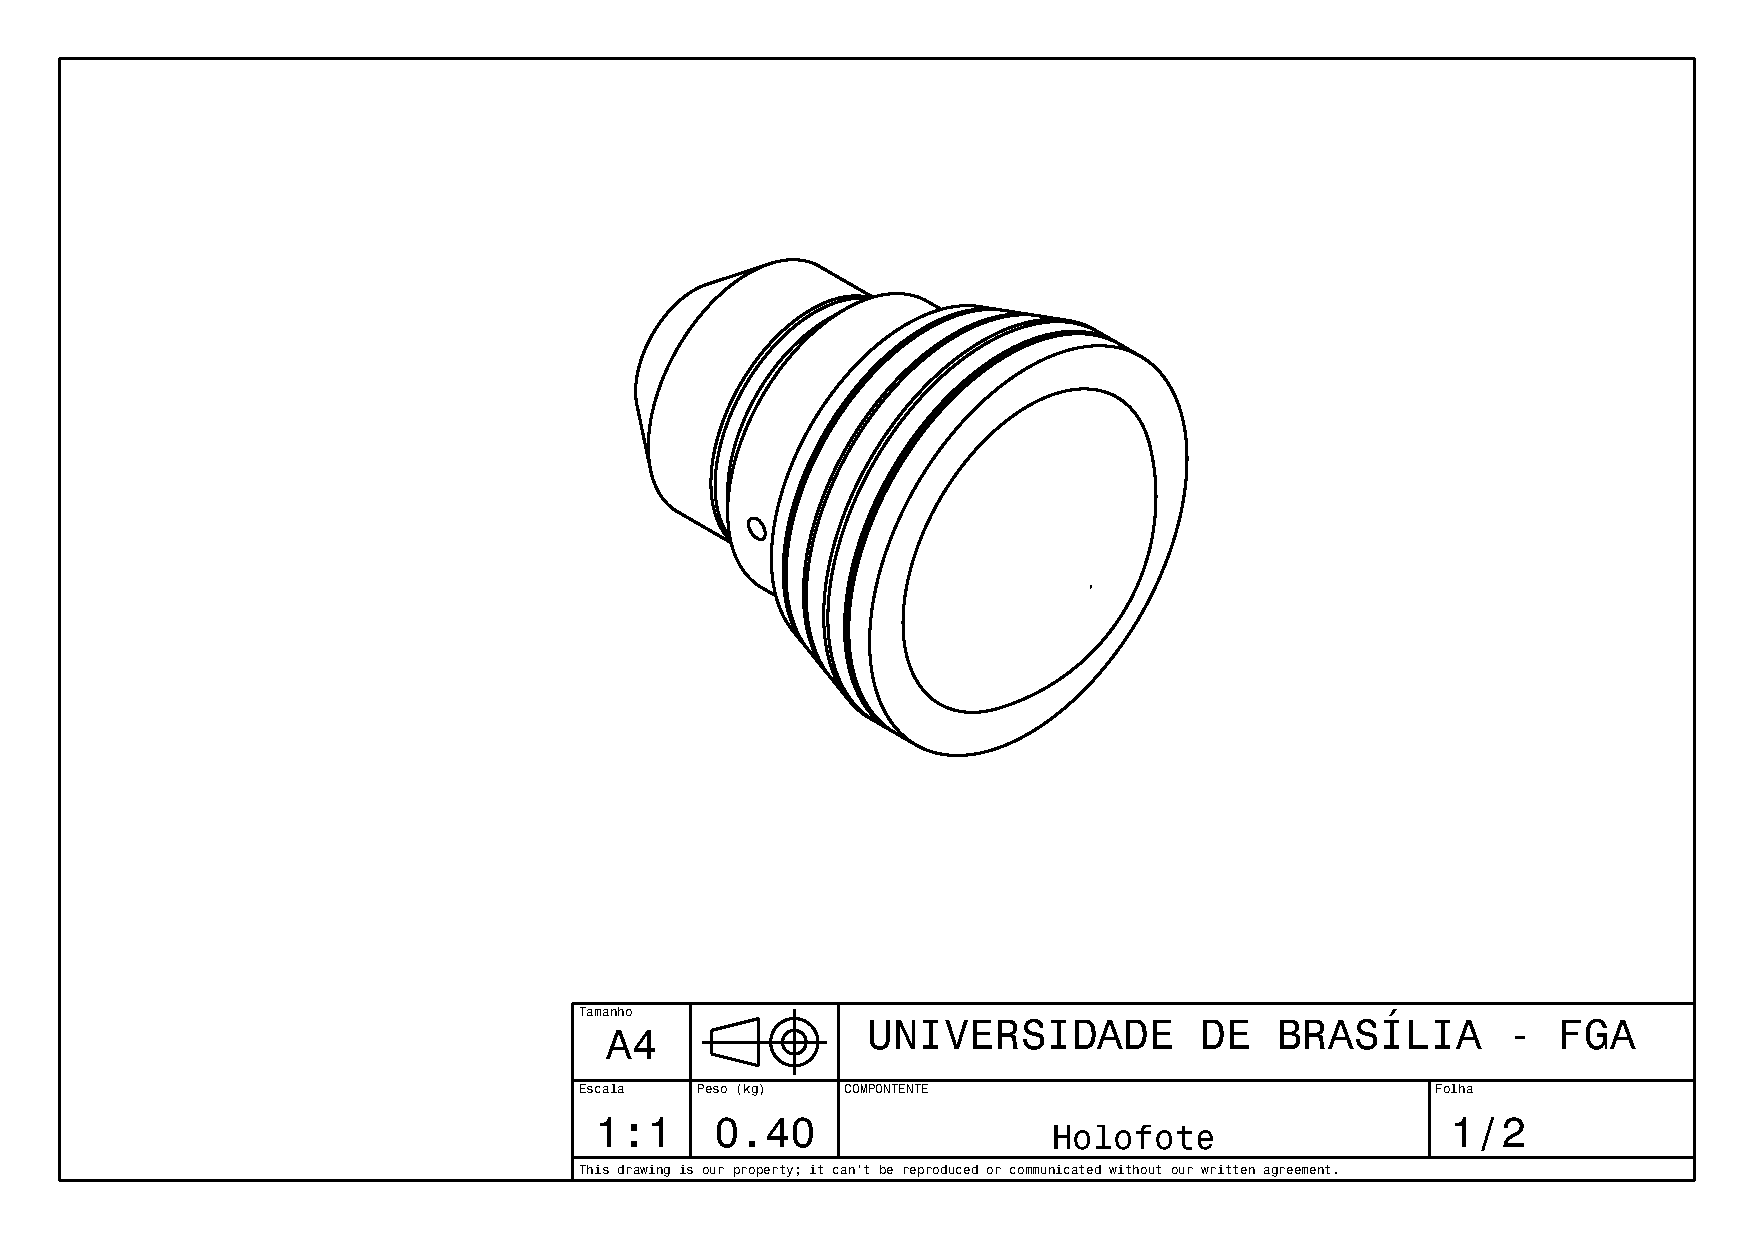
\includepdf[angle=90]{Holofote1.pdf}
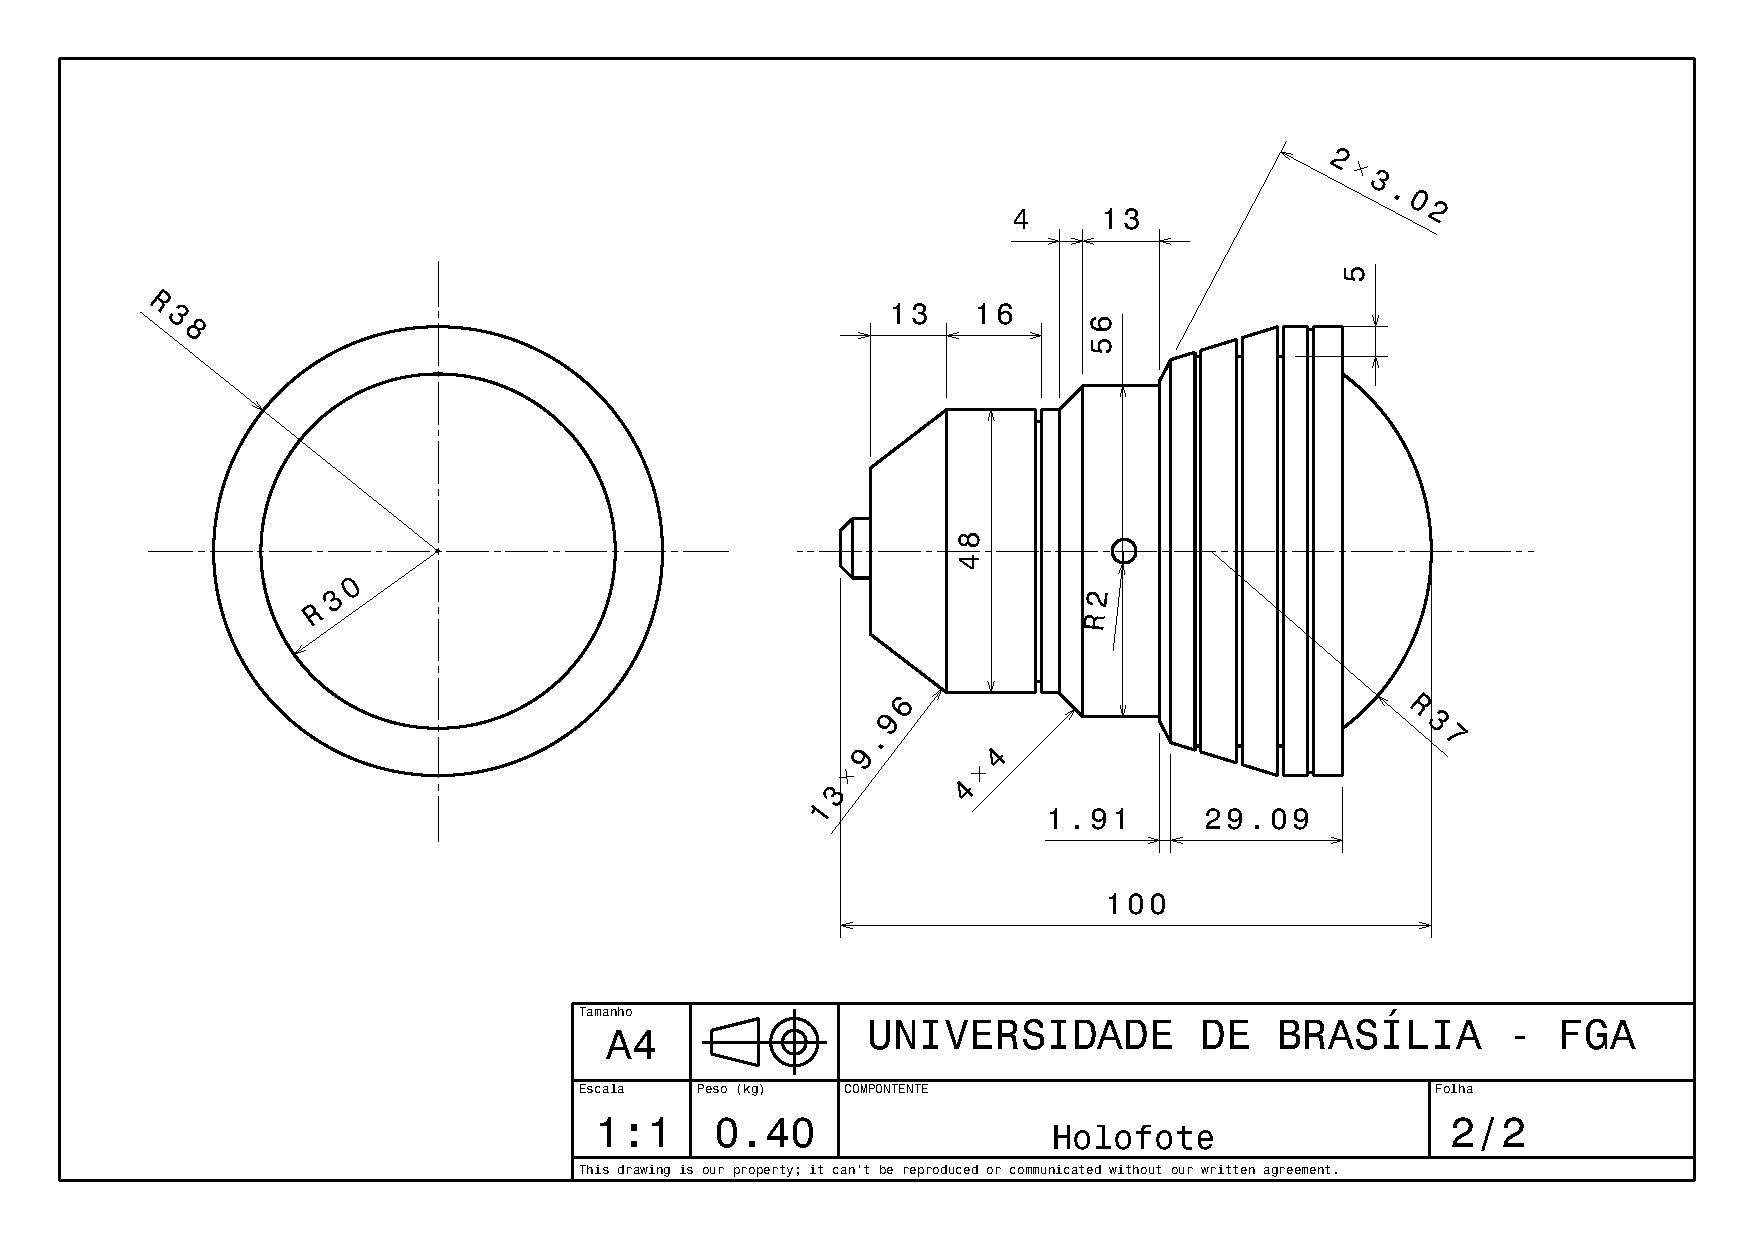
\includepdf[angle=90]{Holofote2.pdf}
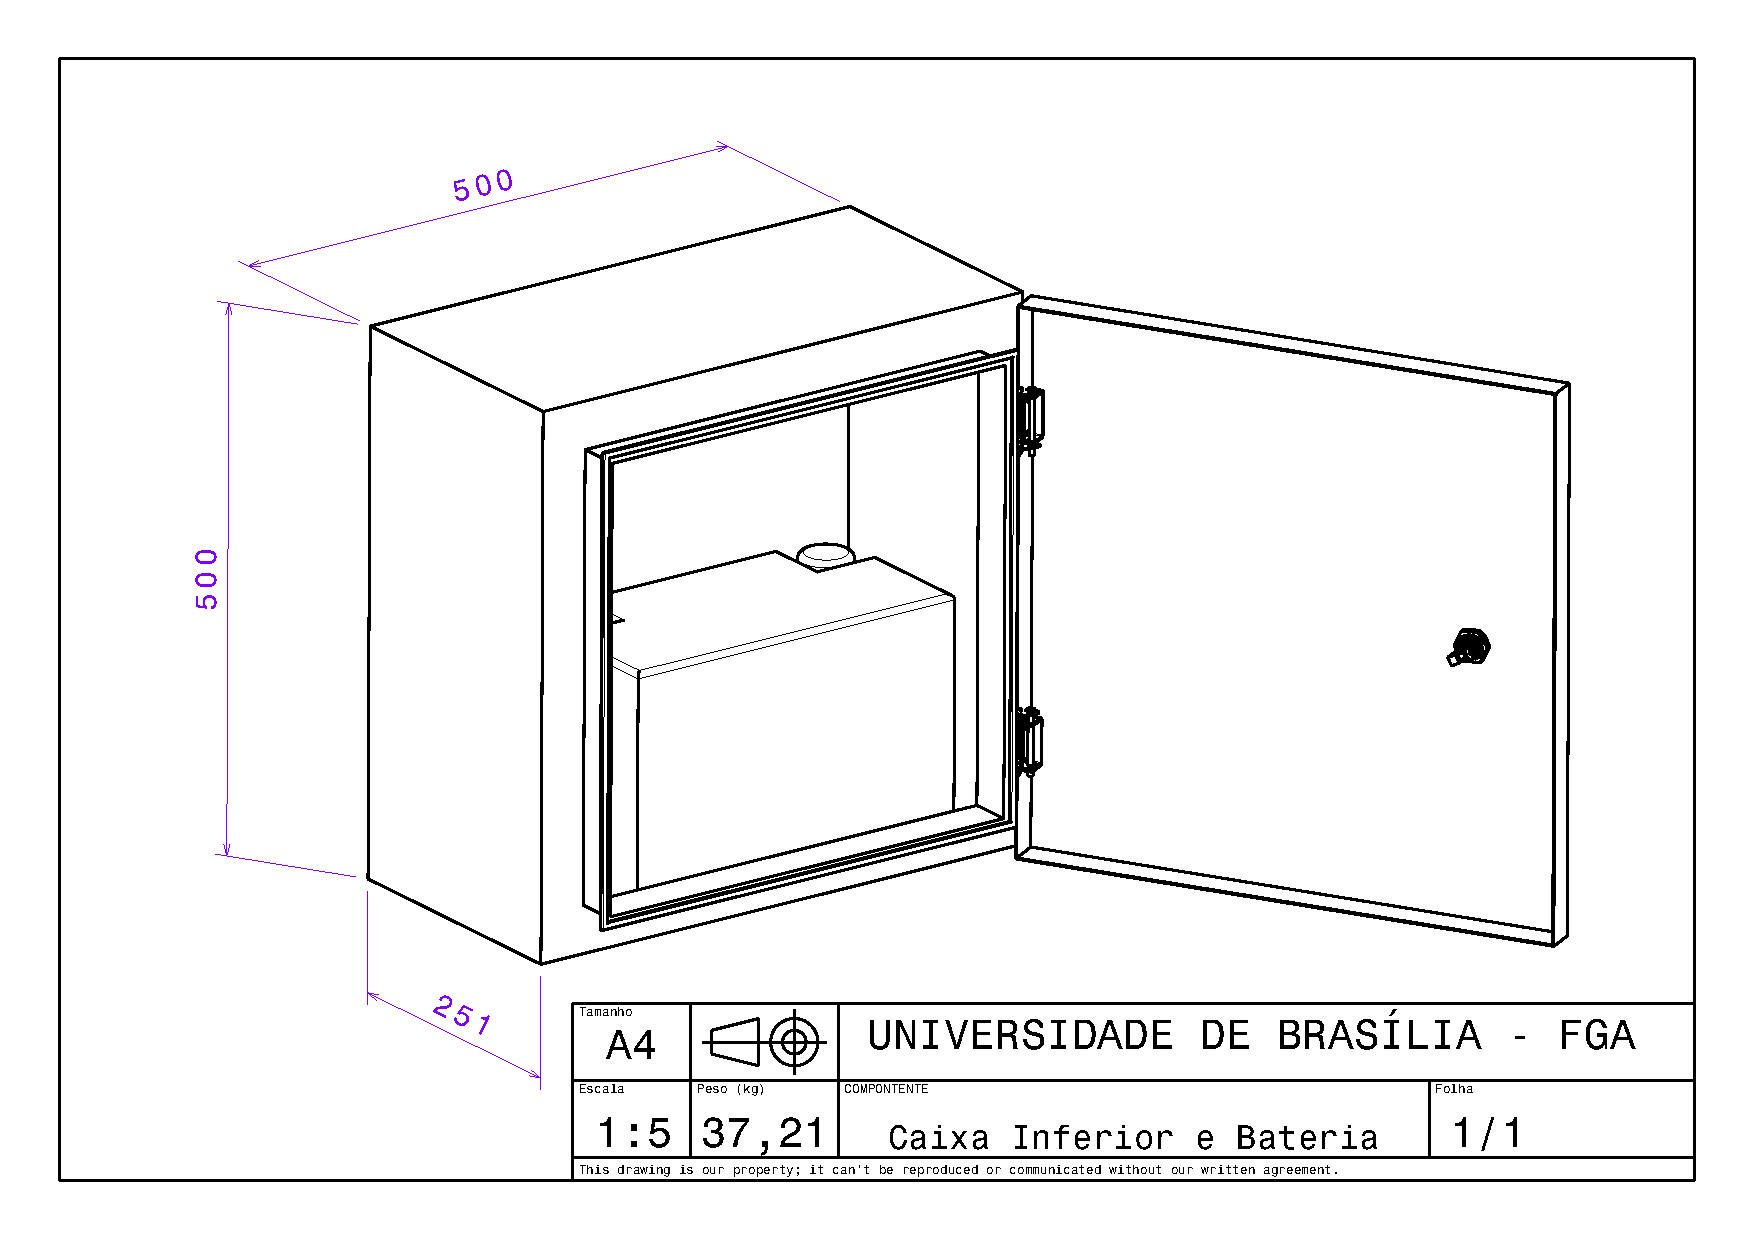
\includepdf[angle=90]{CaixaInf.pdf}
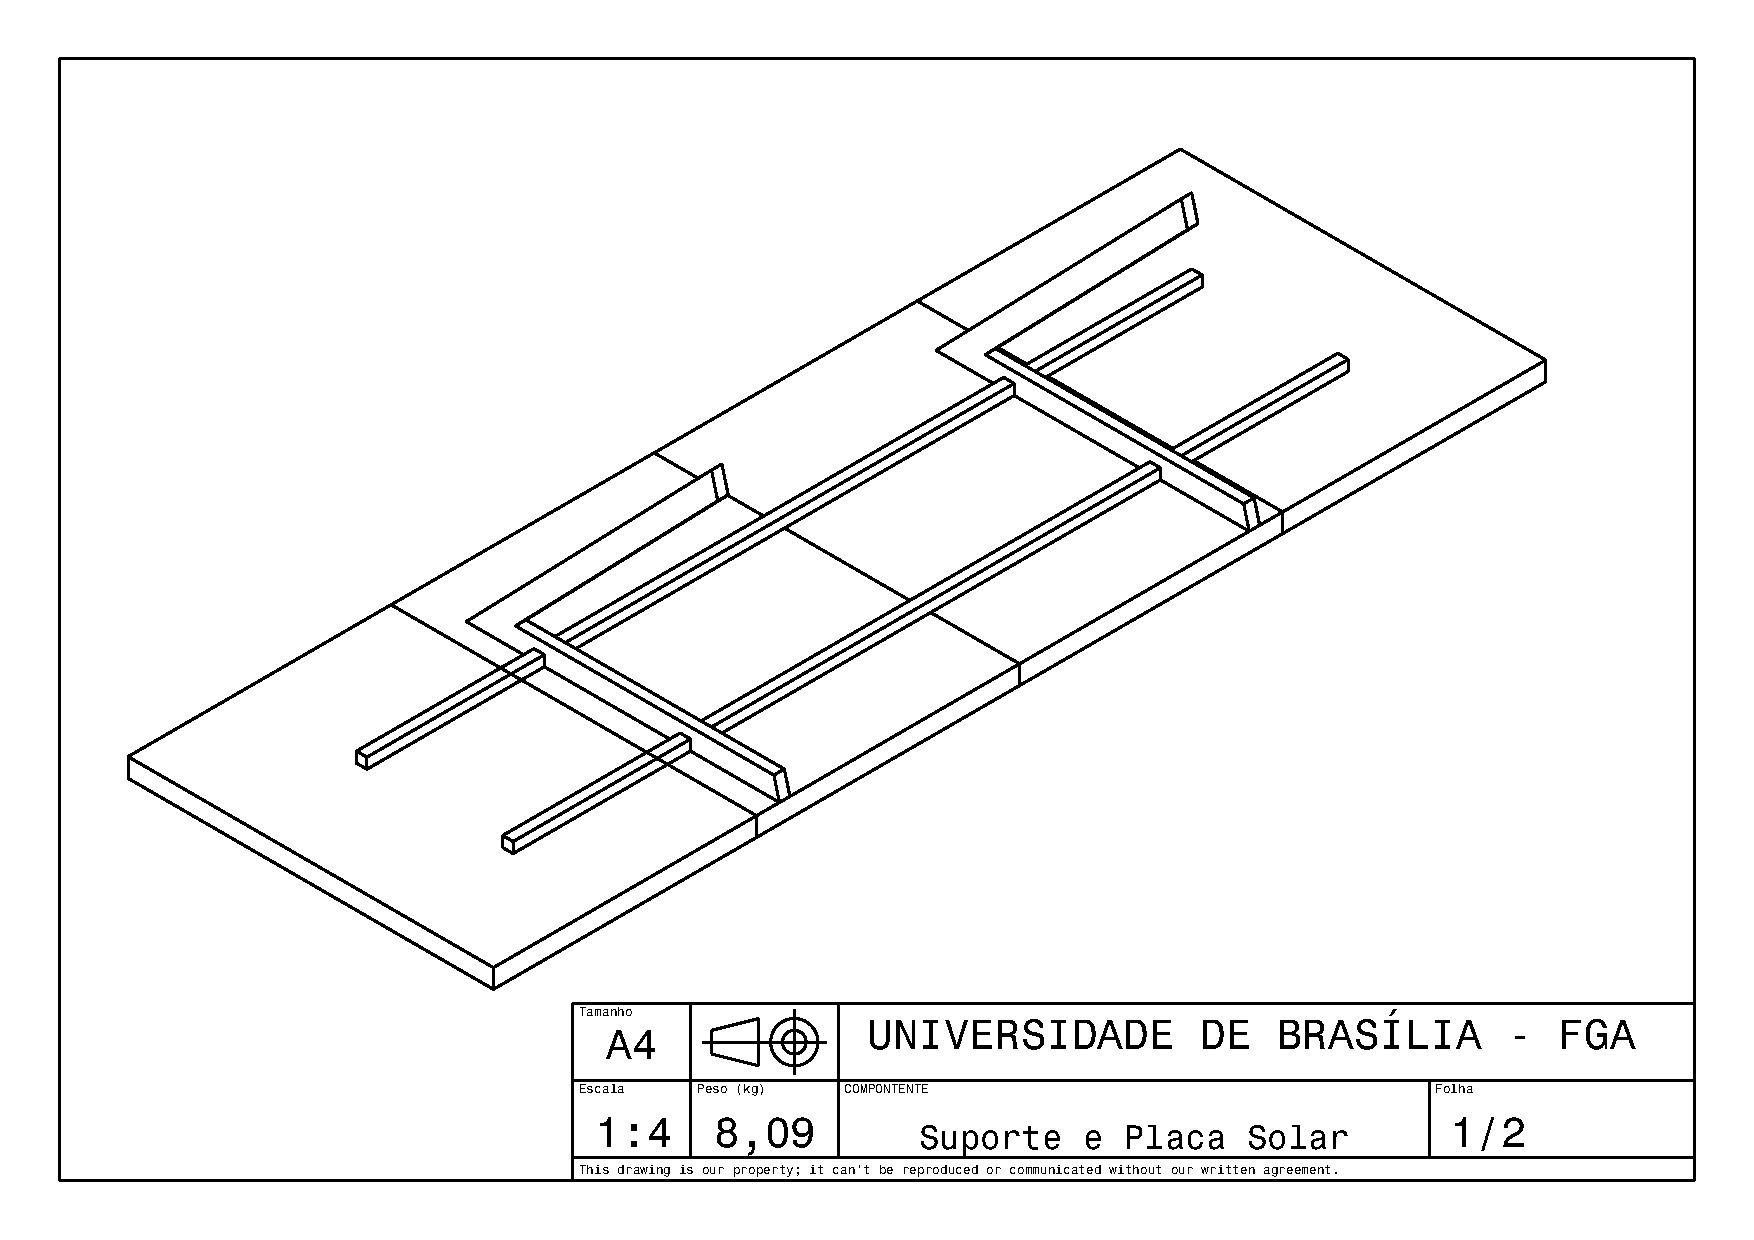
\includepdf[angle=90]{SuportePainel1.pdf}
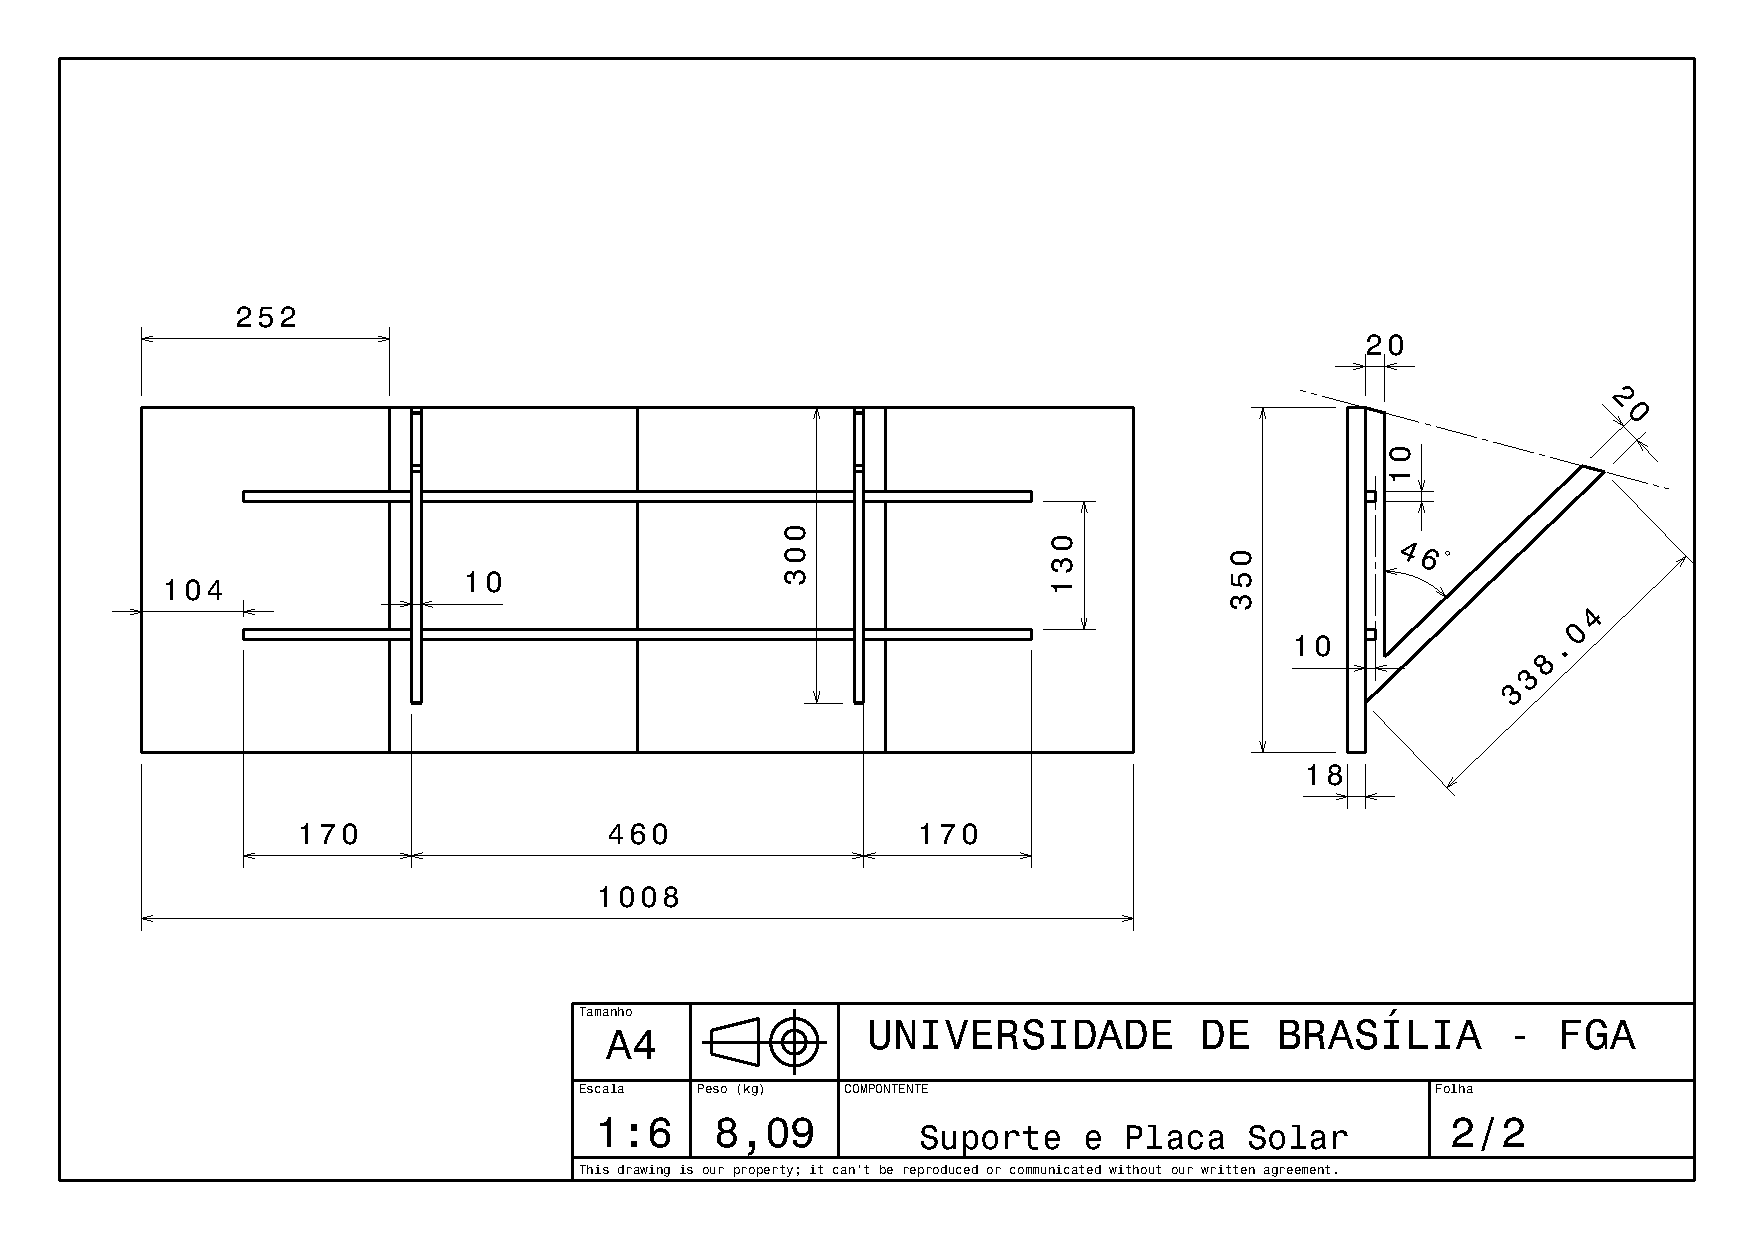
\includepdf[angle=90]{SuportePainel2.pdf}
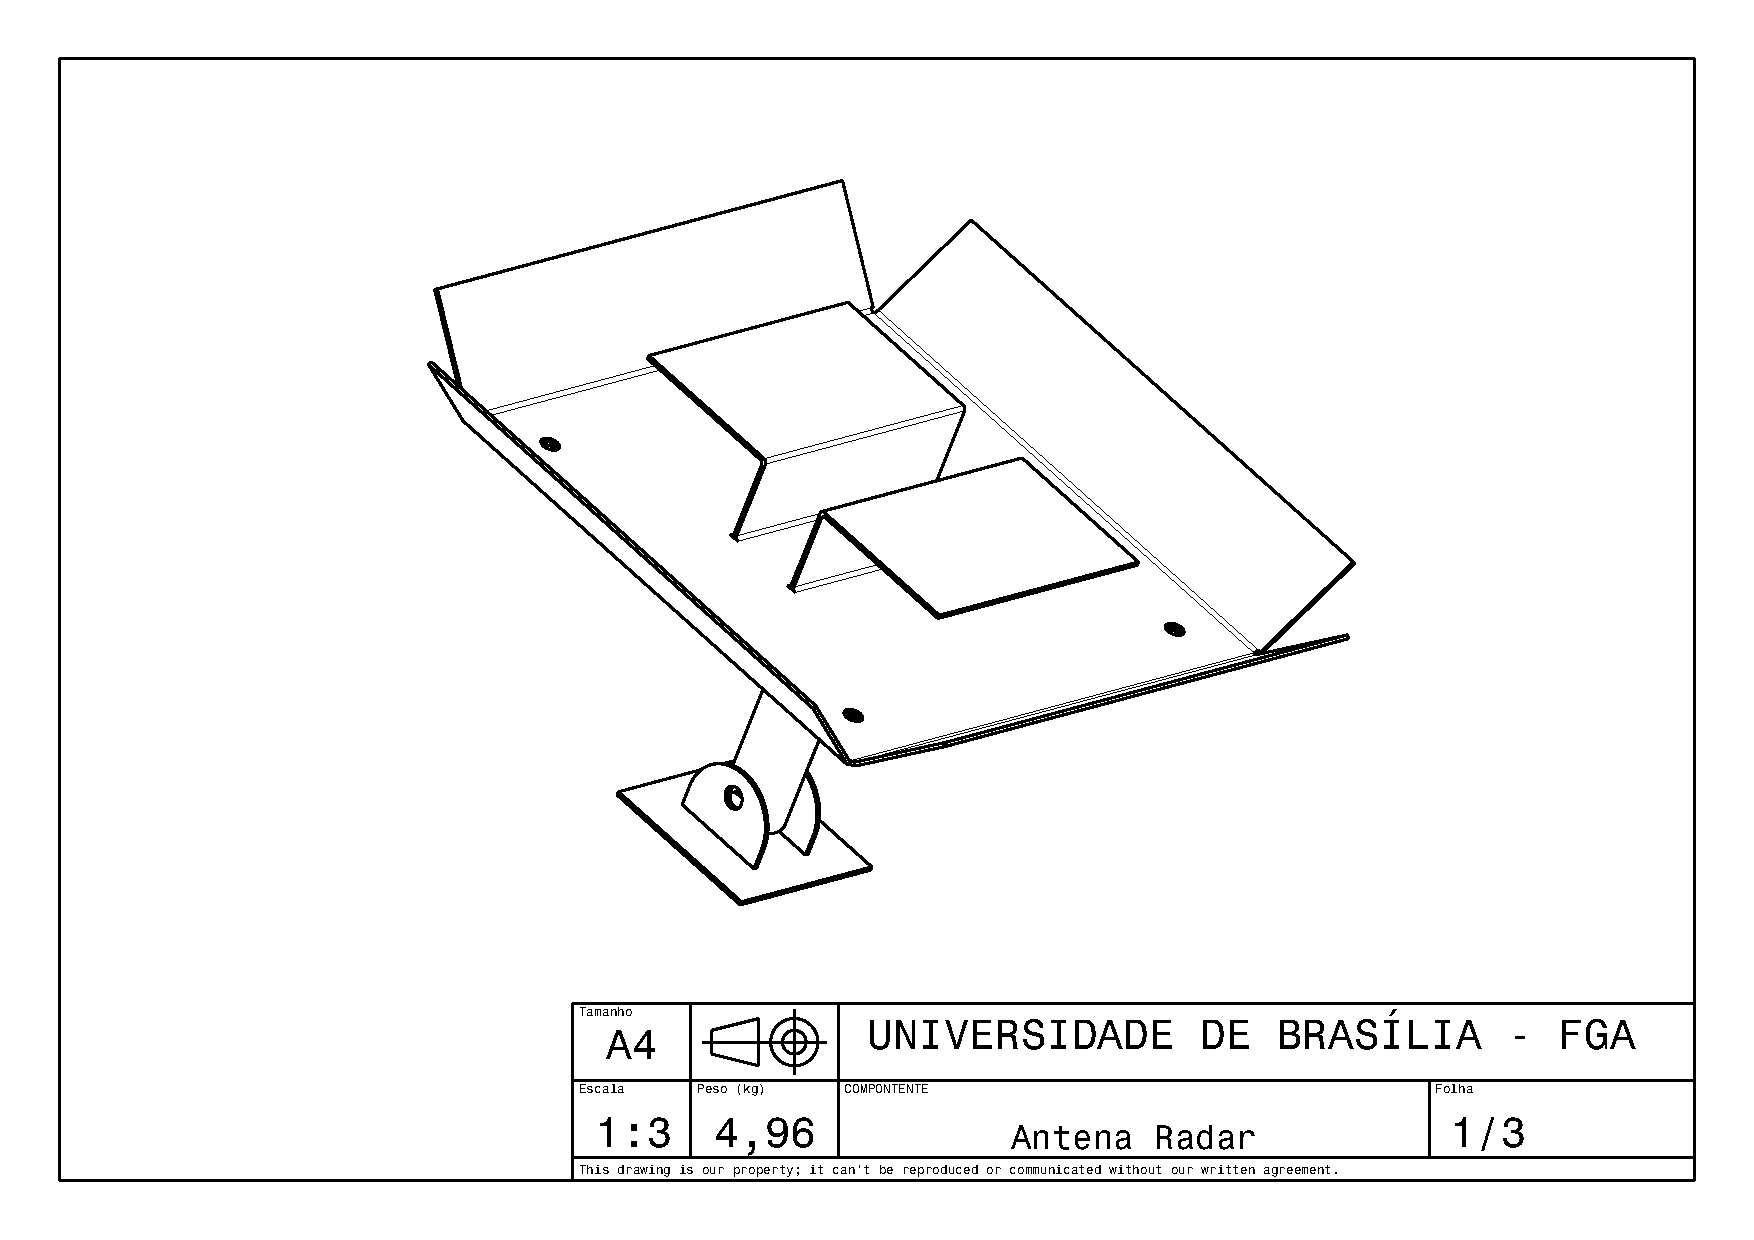
\includepdf[angle=90]{AntenaRadar1.pdf}
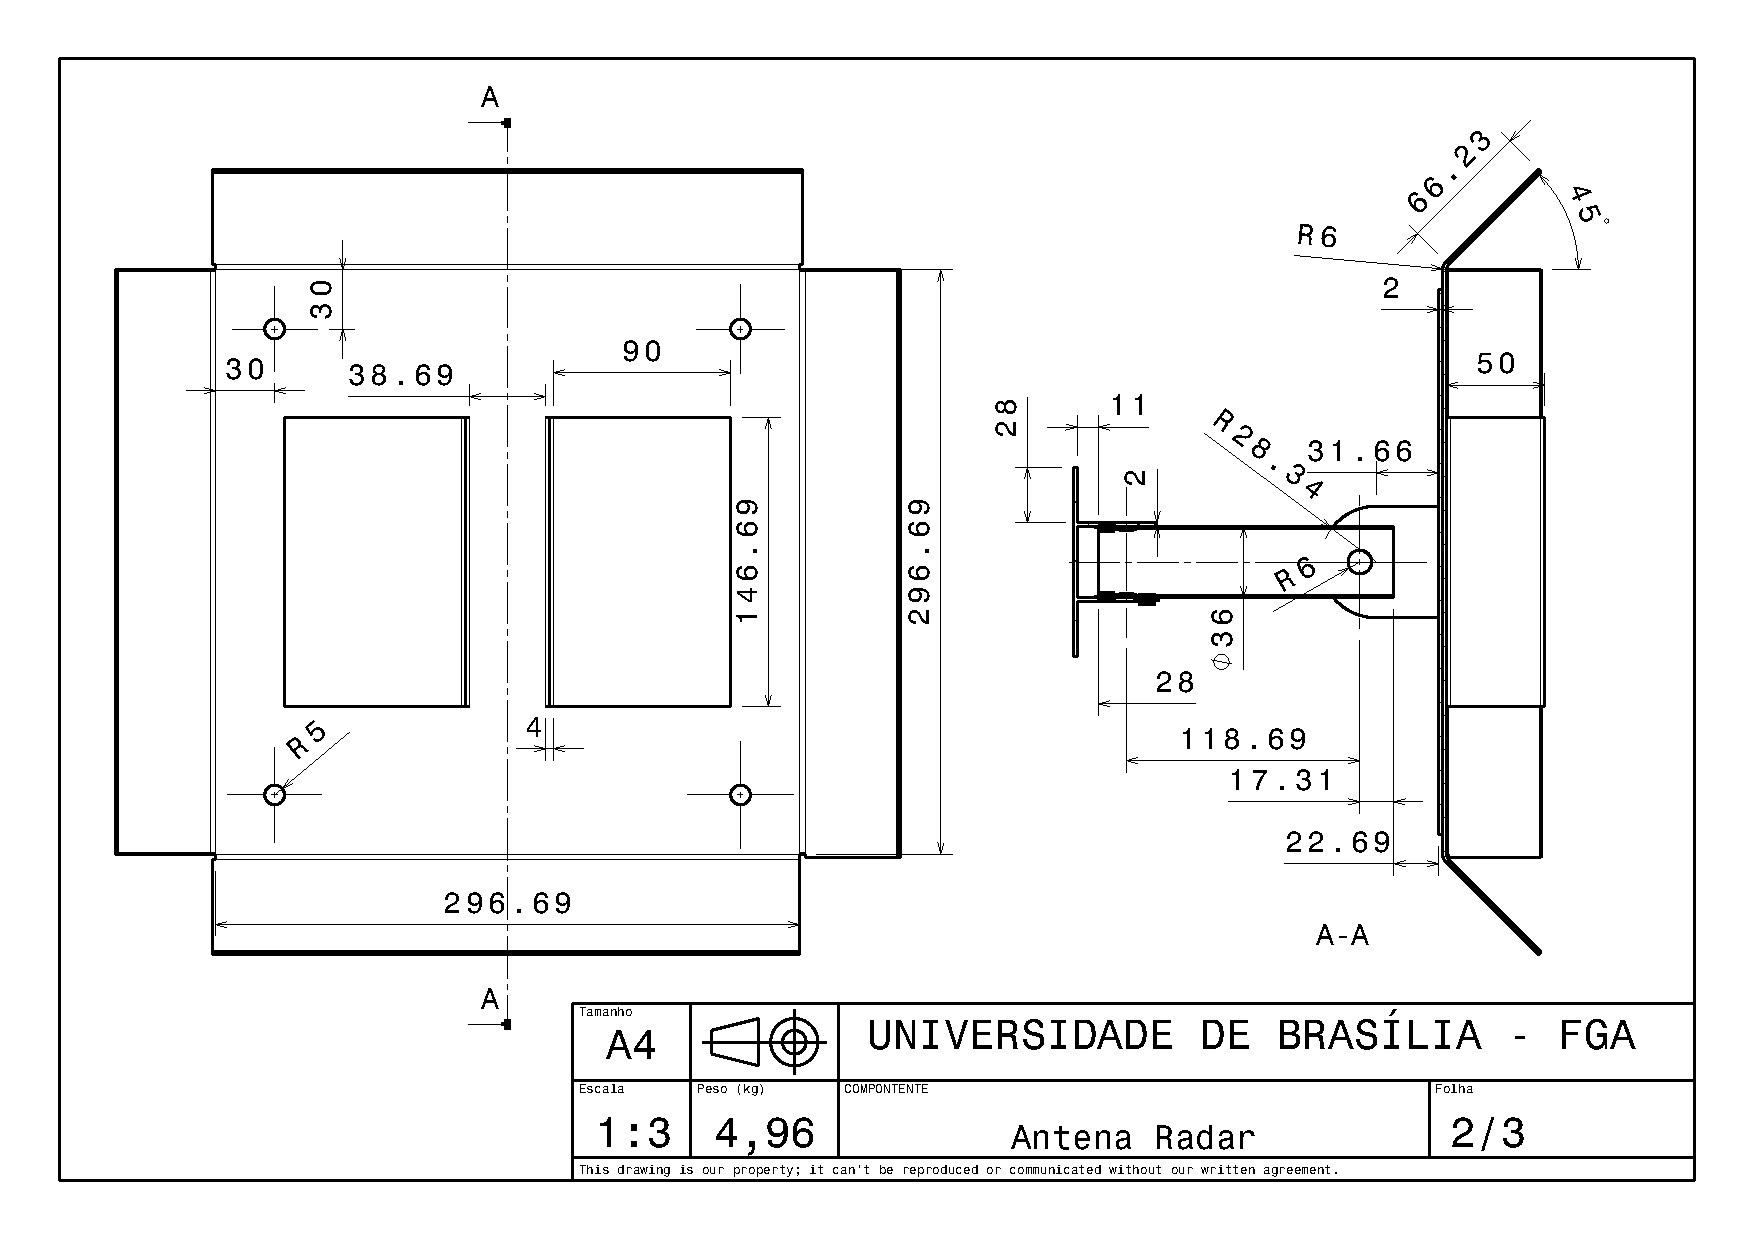
\includepdf[angle=90]{AntenaRadar2.pdf}
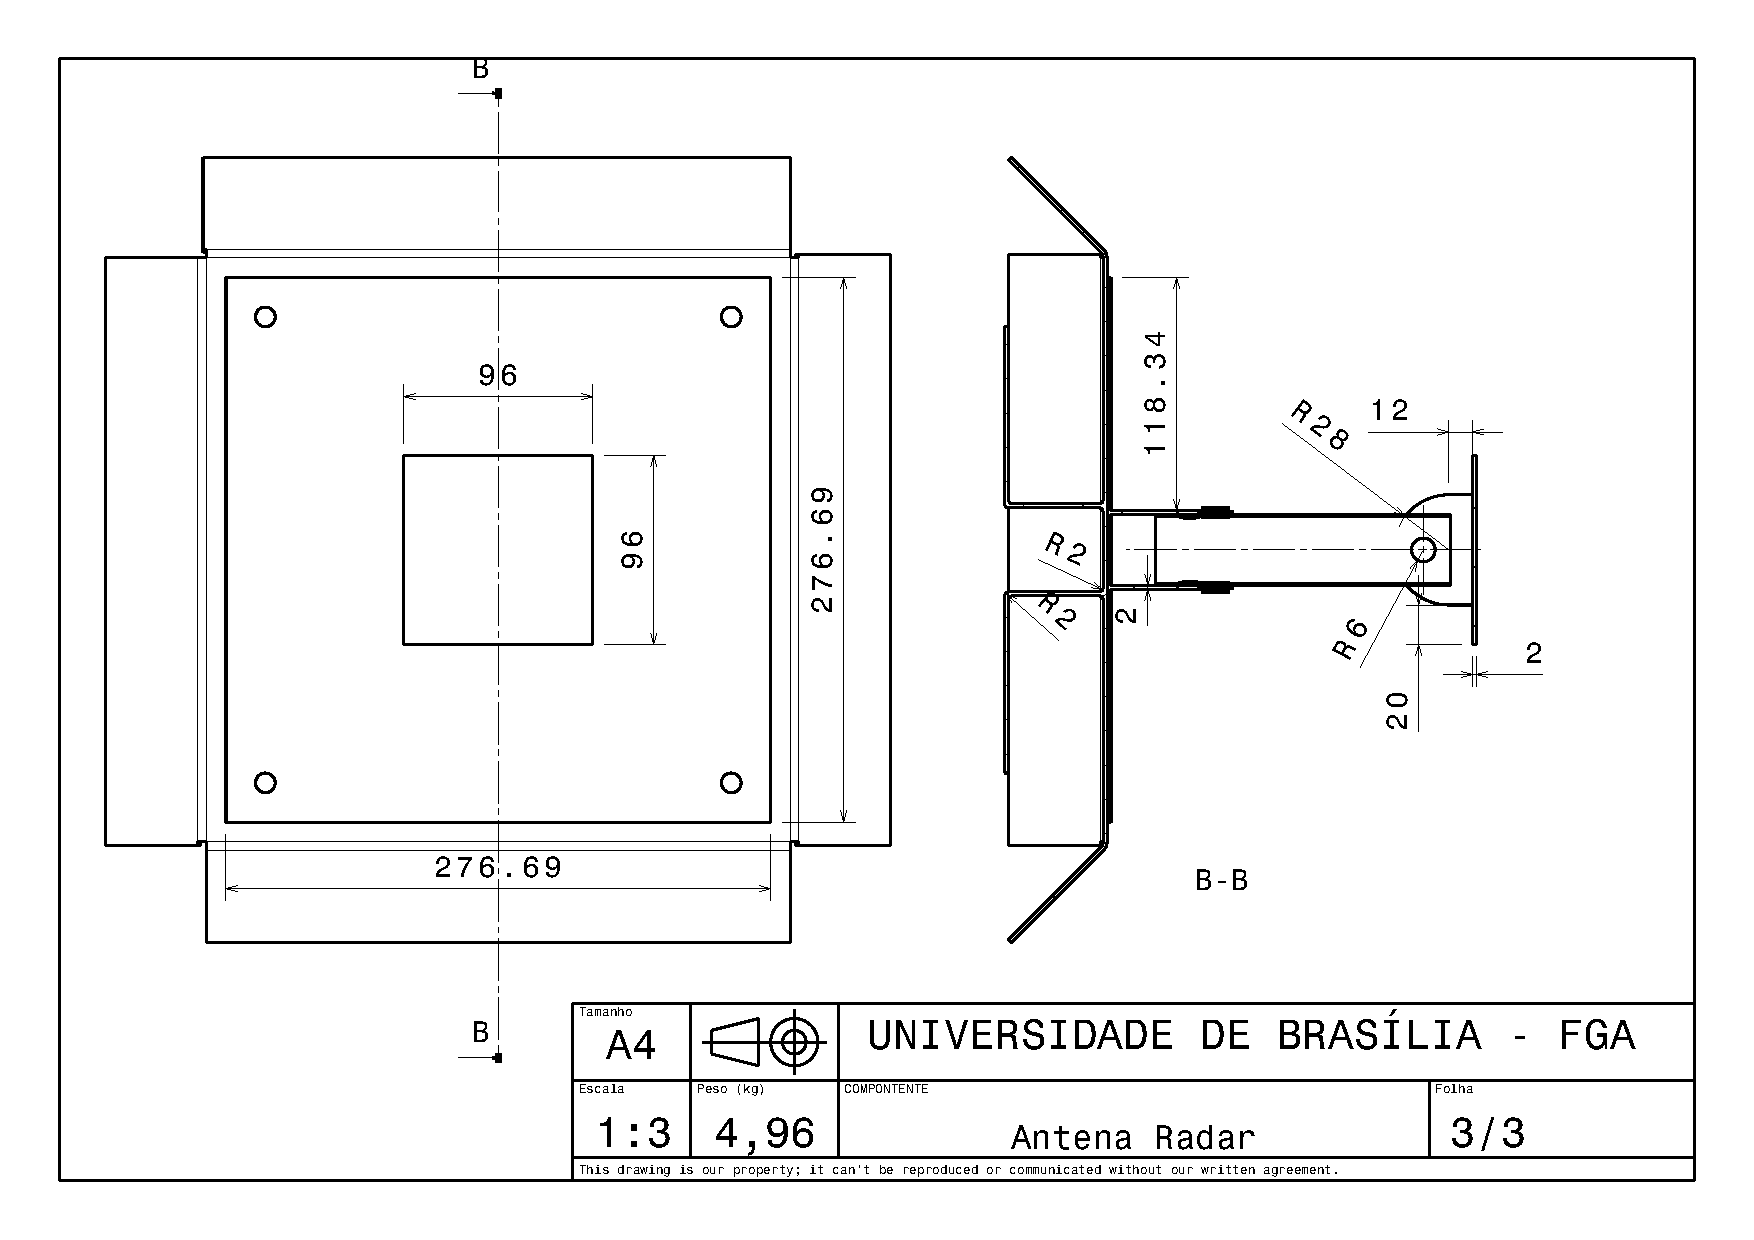
\includepdf[angle=90]{AntenaRadar3.pdf}
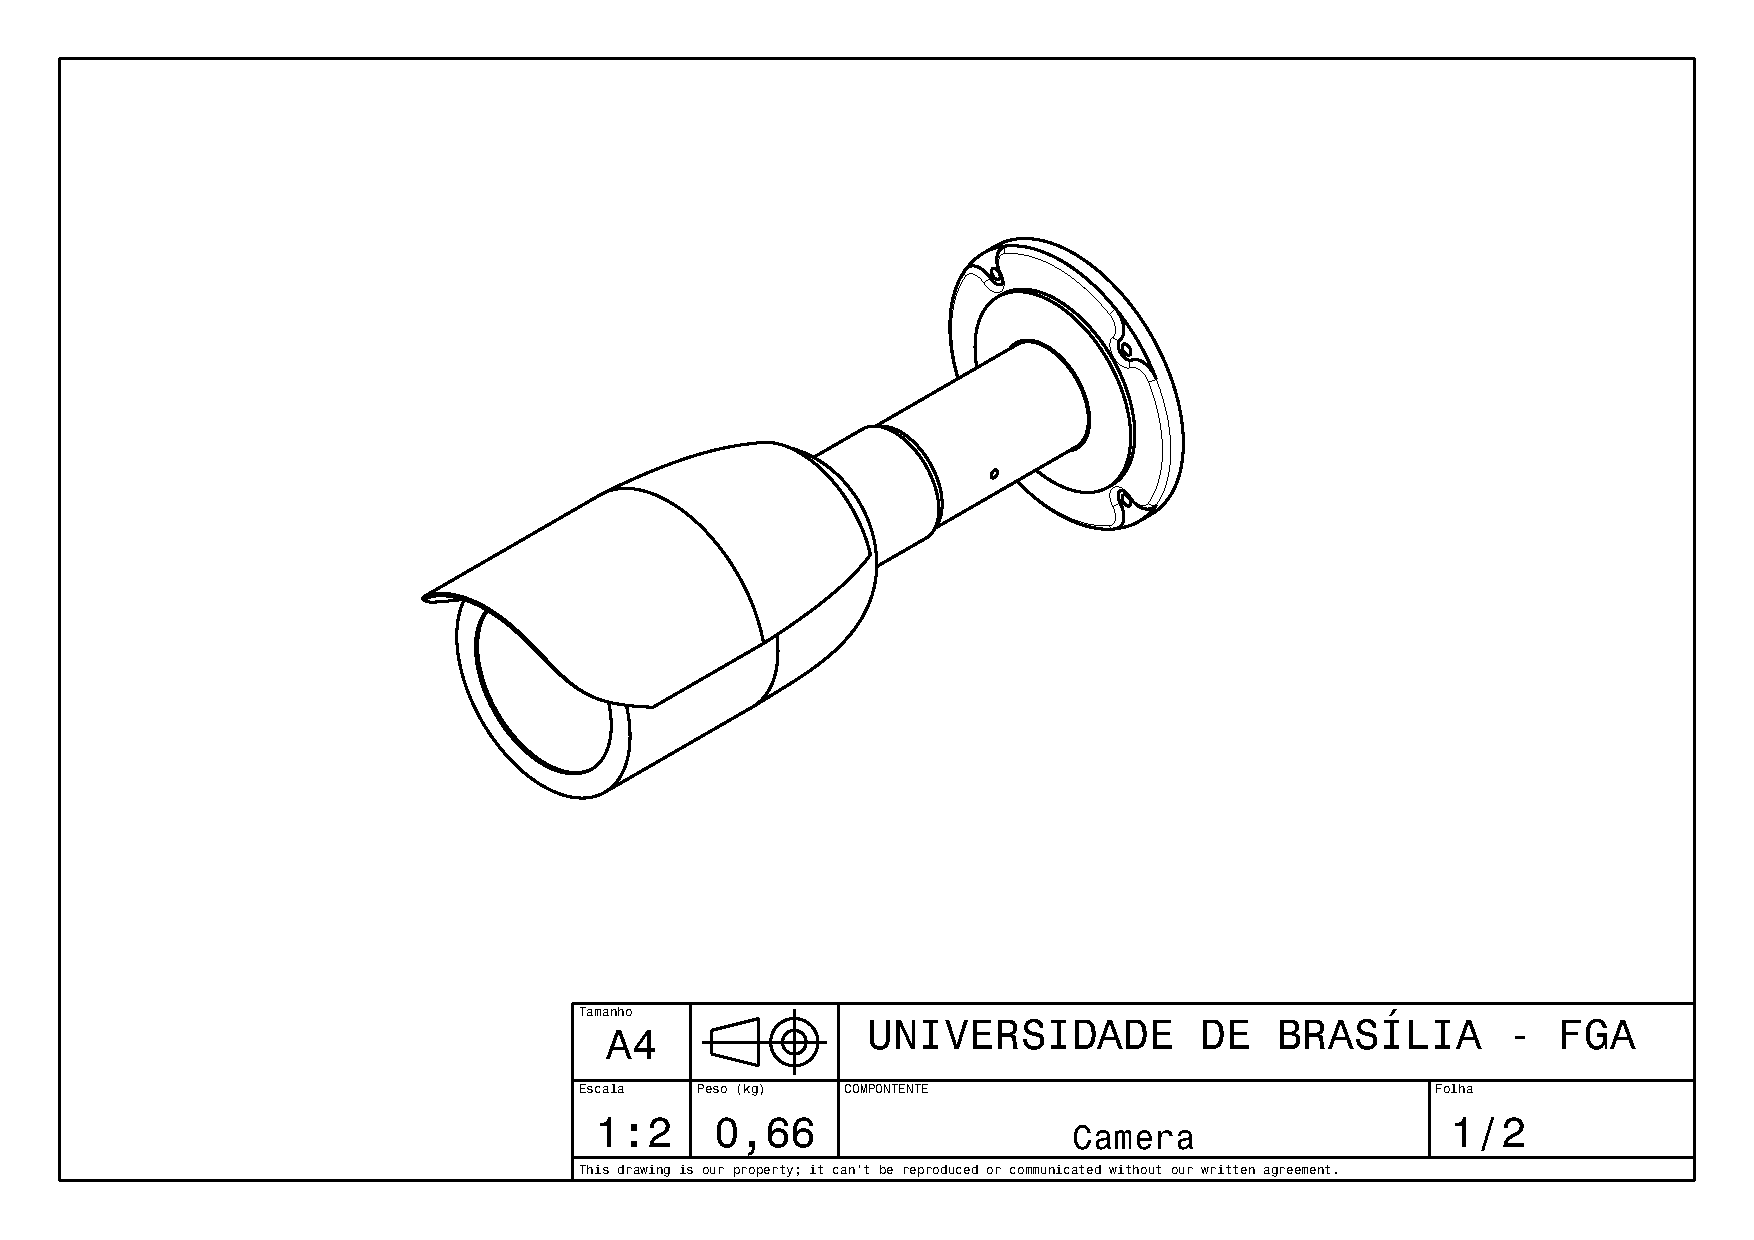
\includepdf[angle=90]{Camera1.pdf}
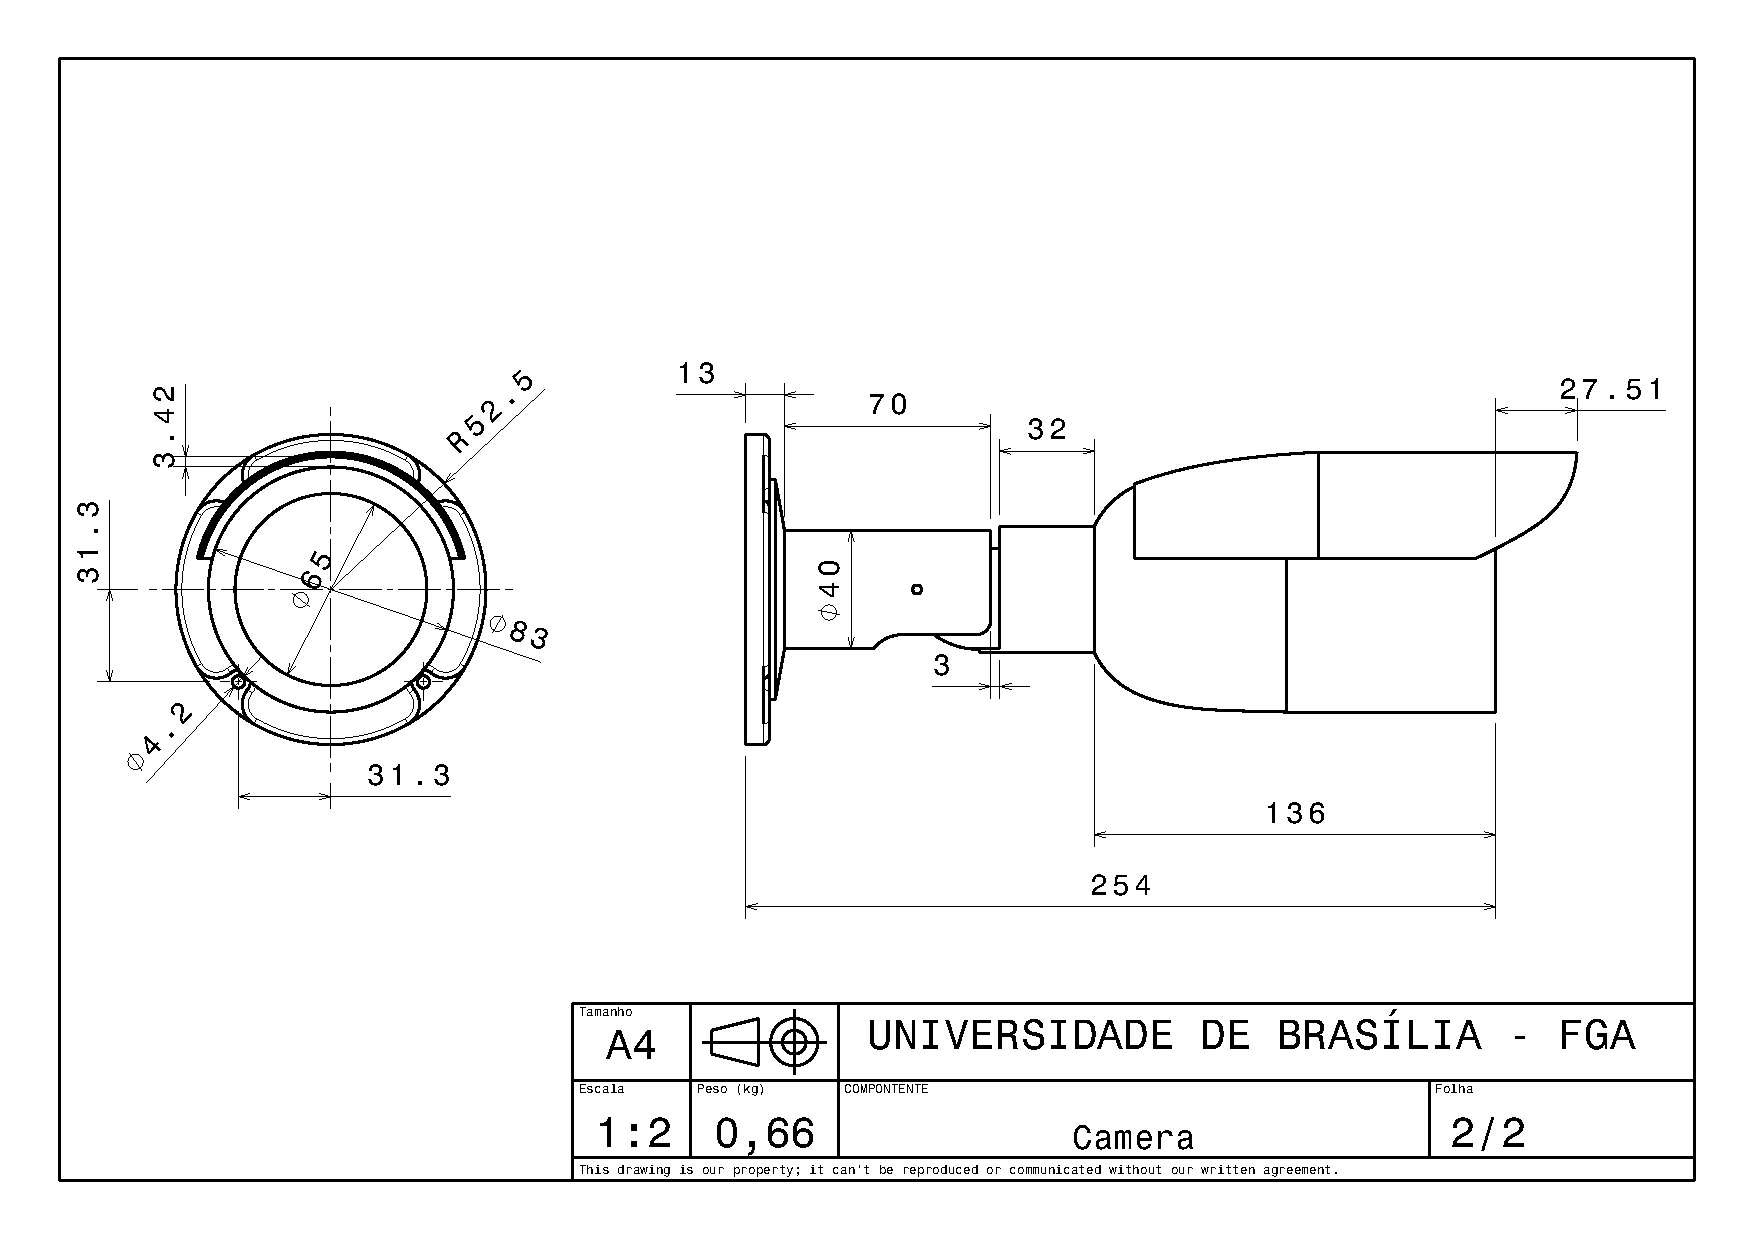
\includepdf[angle=90]{Camera2.pdf}
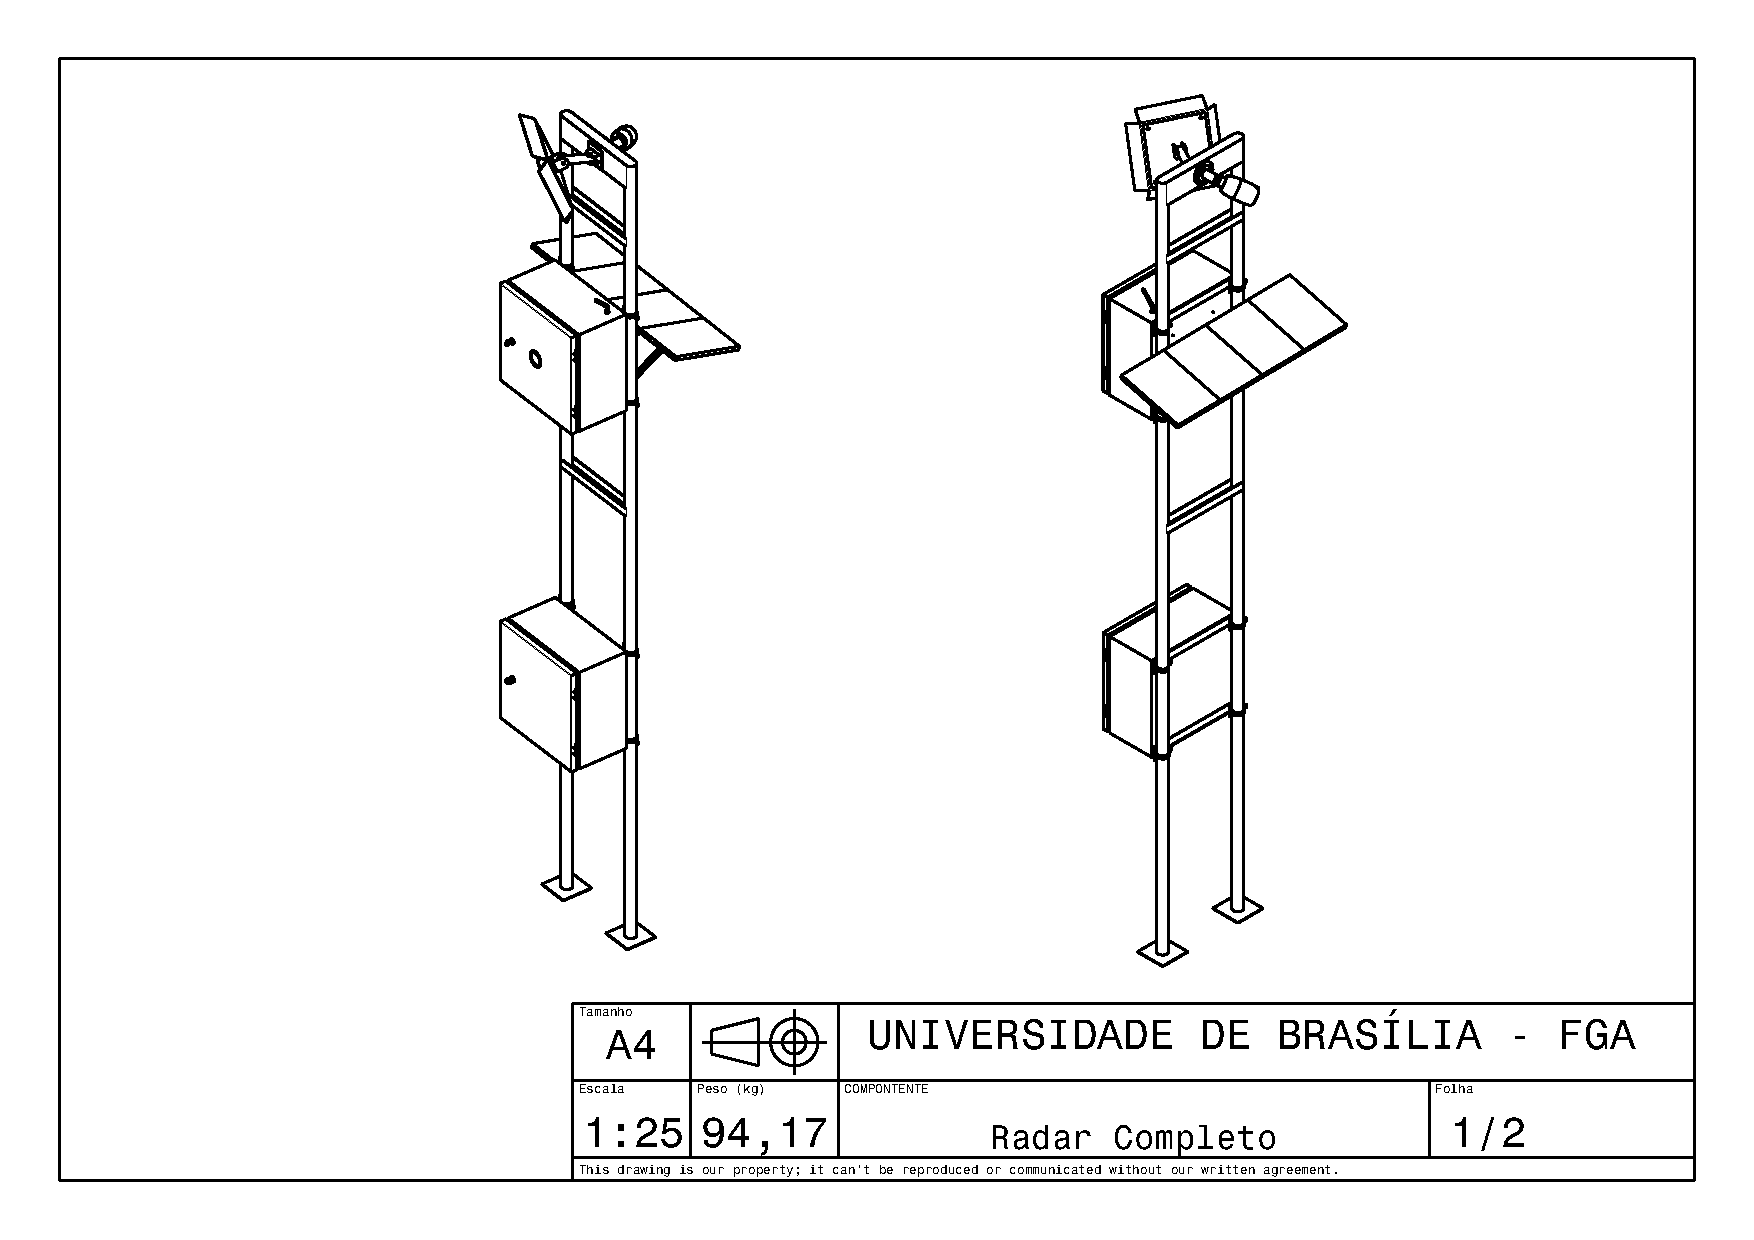
\includepdf[angle=90]{RadarCompleto1.pdf}
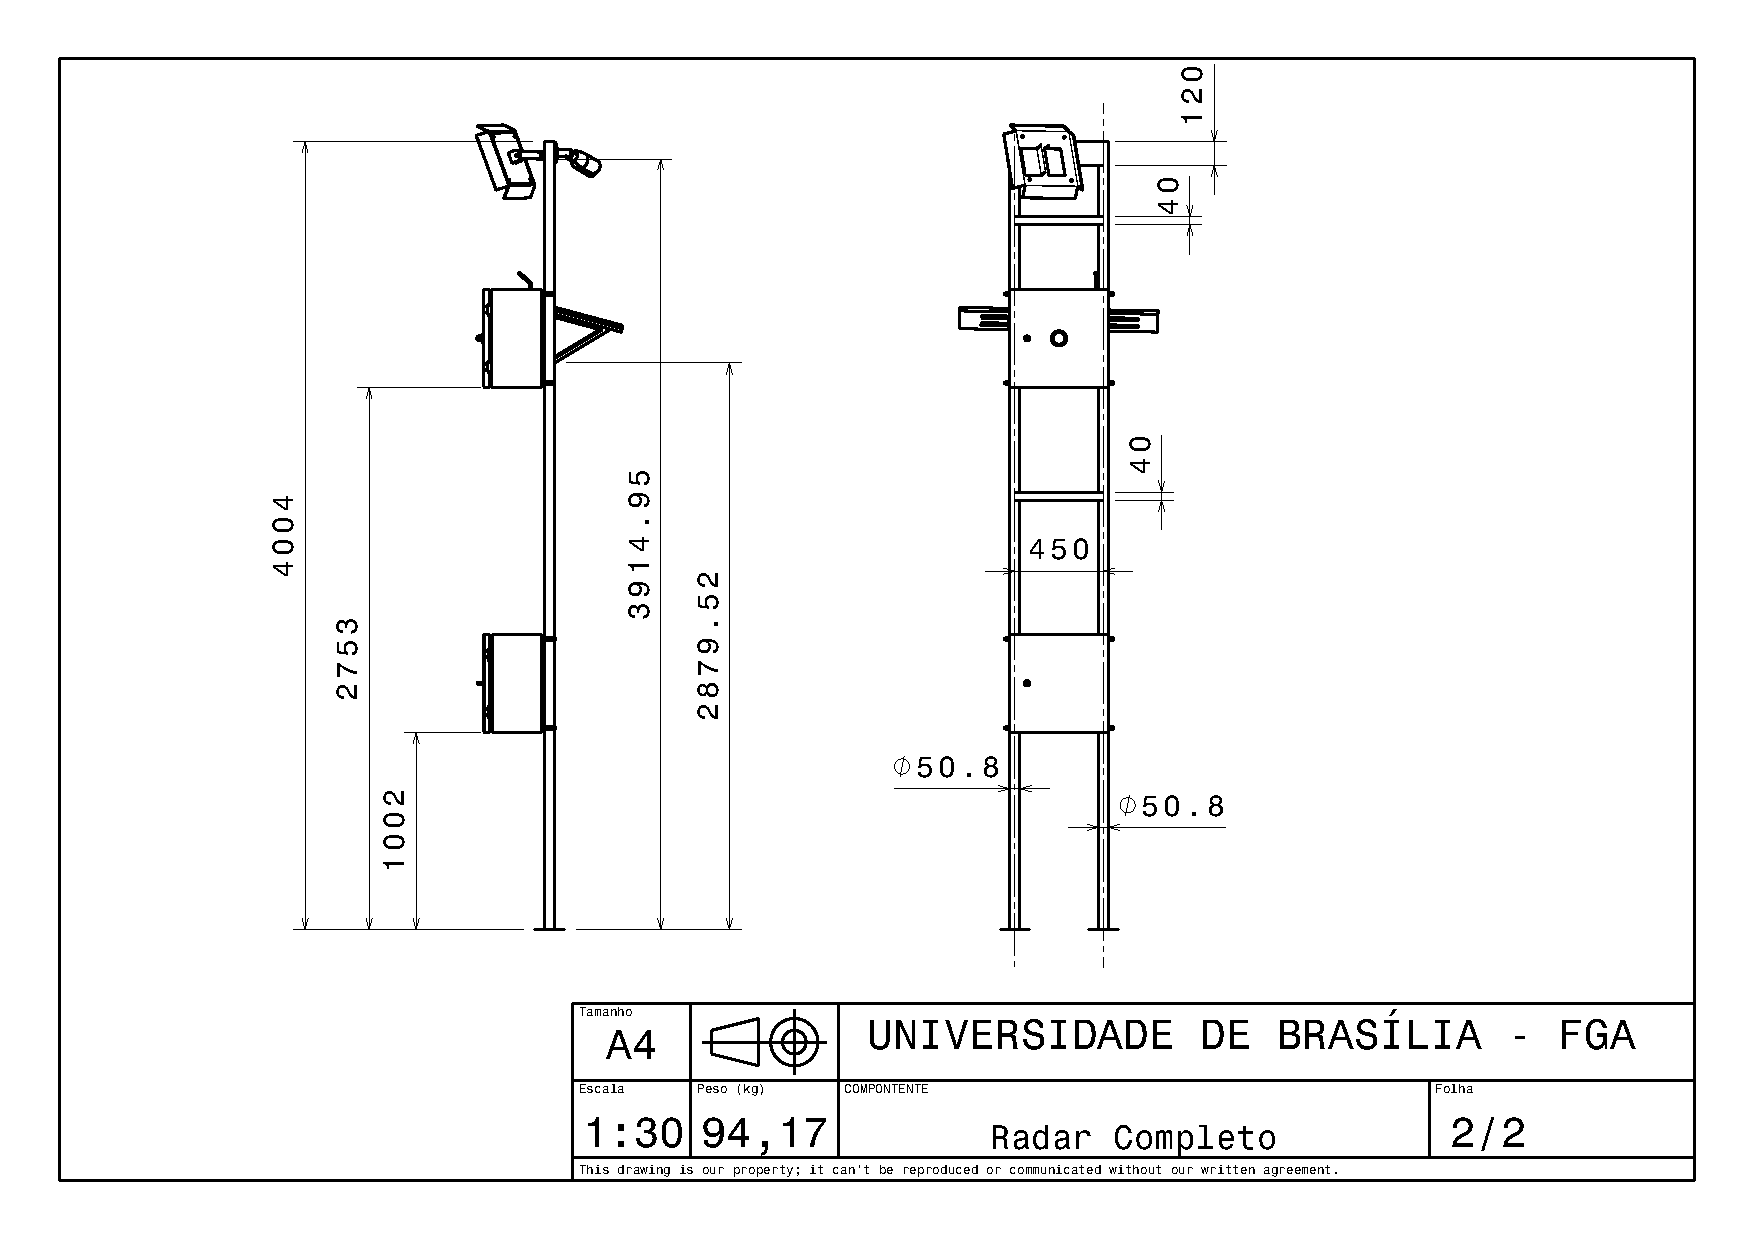
\includepdf[angle=90]{RadarCompleto2.pdf}

\end{anexosenv}

